%----------------------------------------------------------------------------------------
%	PACKAGES AND THEMES
%----------------------------------------------------------------------------------------
\documentclass[aspectratio=169,xcolor=dvipsnames]{beamer}
\usetheme{SimplePlus}

\usepackage{amsmath}

%\usepackage[T1]{fontenc}
\usepackage[utf8]{inputenc}
\usepackage[serbian]{babel}

%\usepackage[T1]{fontenc}

\usepackage{hyperref}
\usepackage{graphicx} % Allows including images
\usepackage{booktabs} % Allows the use of \toprule, \midrule and \bottomrule in tables

%----------------------------------------------------------------------------------------
%	TITLE PAGE
%----------------------------------------------------------------------------------------

\title[short title]{Akvizicija i digitalna obrada signala za eksperimentalnu analizu dinamike sistema spregnutih klatana} % The short title appears at the bottom of every slide, the full title is only on the title page
\subtitle{Master rad}


\author {Mentor: Prof. Dr Vladimir Rajović
\qquad\qquad
\hfill Kandidat: David Milovanović
}


\institute[NTU] % Your institution as it will appear on the bottom of every slide, may be shorthand to save space
{
    Univerzitet u Beogradu \\
    Elektrotehnički fakultet % Your institution for the title page
}
\date{\today} % Date, can be changed to a custom date
%\date{28. septembar, 2022}


%----------------------------------------------------------------------------------------
%	PRESENTATION SLIDES
%----------------------------------------------------------------------------------------

\begin{document}

\begin{frame}
    % Print the title page as the first slide
    \titlepage
\end{frame}

\begin{frame}{Pregled}
    % Throughout your presentation, if you choose to use \section{} and \subsection{} commands, these will automatically be printed on this slide as an overview of your presentation
    \tableofcontents
\end{frame}

%------------------------------------------------
\section{Teorijski uvod}
%------------------------------------------------

\begin{frame}
    \Huge{\centerline{\textbf{Teorijski uvod}}}
\end{frame}
%------------------------------------------------


\subsection{Oscilacije}

\begin{frame}{Oscilacije}
    \begin{figure}
    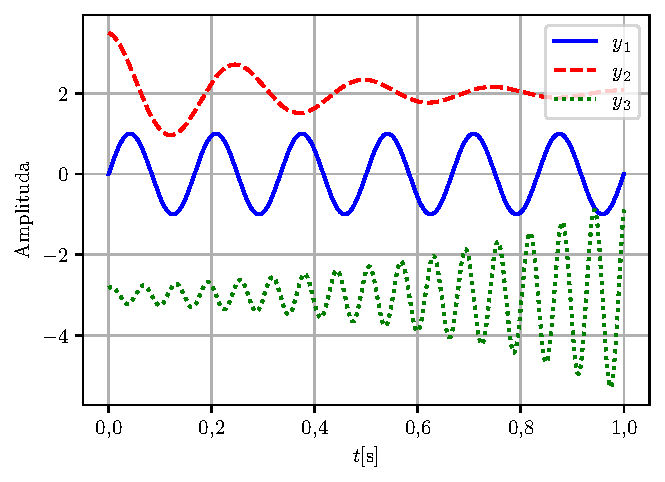
\includegraphics[width=0.5\linewidth]{master_fig/osc_py.pdf}
    \caption{Tipovi oscilacija.}
    \end{figure}
\end{frame}

%------------------------------------------------
\subsection{Oscilatori}

\begin{frame}{Oscilatori}
	\begin{columns}[c]
    \begin{column}{.5\textwidth}
    \begin{figure}
        \centering
        
\includegraphics[width=0.9\textwidth]{master_fig/dva_odvojena_osc.pdf}
        \caption{Dva odvojena oscilatora.}
    \end{figure}      
    \end{column}
    \begin{column}{.5\textwidth}
    \begin{figure}
        \centering
        
\includegraphics[width=0.9\textwidth]{master_fig/spregnuti_osc.pdf}
        \caption{Dva spregnuta oscilatora.}
    \end{figure}
    \end{column}
\end{columns}
	
\end{frame}

%------------------------------------------------



\subsection{Klatno}

\begin{frame}{Klatno}
    \begin{figure}
    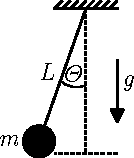
\includegraphics[width=0.3\linewidth]{master_fig/mat_klatno.pdf}
    \caption{Primer klatna.}
    \end{figure}
\end{frame}

%------------------------------------------------

\begin{frame}{Spregnuta klatna}
    \begin{columns}[c]
    \begin{column}{.5\textwidth}
    \begin{figure}
        \centering
        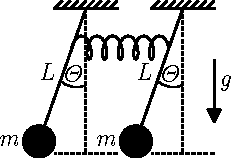
\includegraphics[width=0.9\textwidth]{master_fig/spregnuto_klatno_1.pdf}
        \caption{Mod simetrije.}
    \end{figure}      
    \end{column}
    \begin{column}{.5\textwidth}
    \begin{figure}
        \centering
        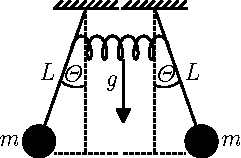
\includegraphics[width=0.9\textwidth]{master_fig/spregnuto_klatno_2.pdf}
        \caption{Mod antisimetrije.}
    \end{figure}
    \end{column}
\end{columns}
\end{frame}

%------------------------------------------------

\subsection{Očekivani teorijski rezultati}

\begin{frame}{Očekivani teorijski rezultati}
    \begin{figure}
    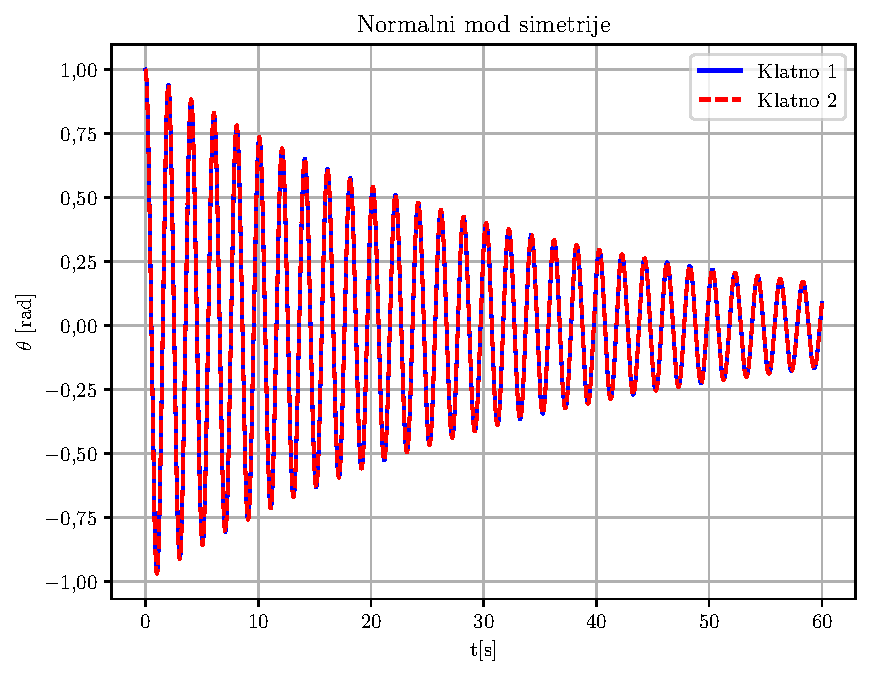
\includegraphics[width=0.5\linewidth]{master_fig/nmod_simetrija.pdf}
    \caption{Teorijski očekivani rezultati moda simetrije.}
    \end{figure}
\end{frame}

%------------------------------------------------

\begin{frame}{Očekivani teorijski rezultati}
    \begin{figure}
    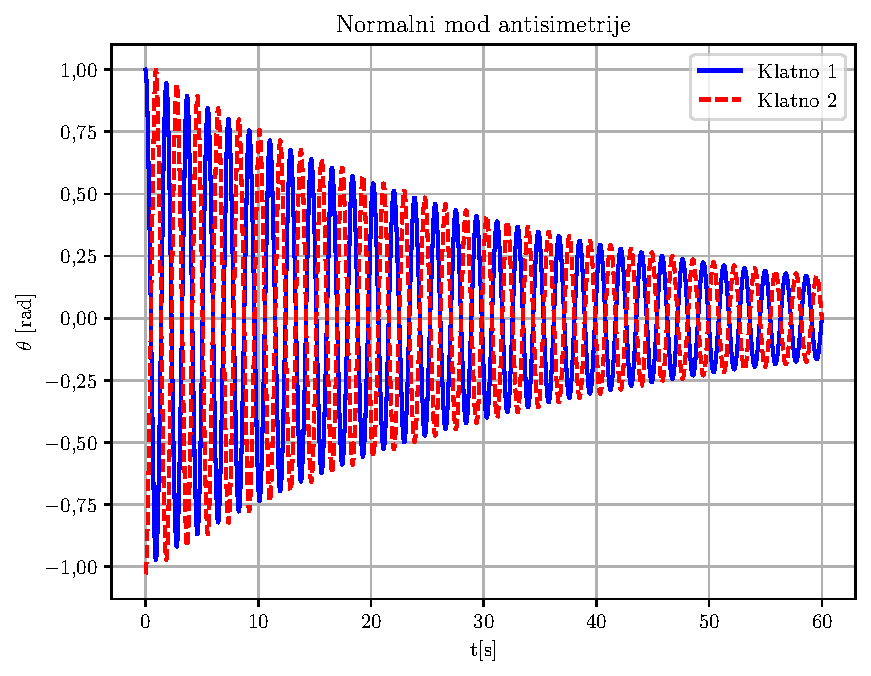
\includegraphics[width=0.5\linewidth]{master_fig/nmod_asimetrija.pdf}
    \caption{Teorijski očekivani rezultati moda antisimetrije.}
    \end{figure}
\end{frame}

%------------------------------------------------

\begin{frame}{Očekivani teorijski rezultati}
    \begin{figure}
    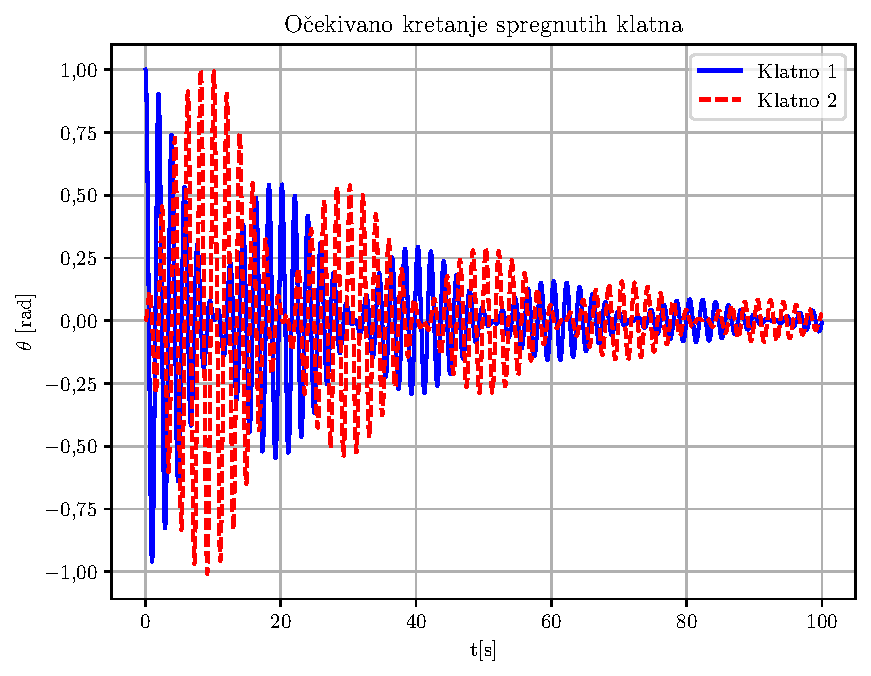
\includegraphics[width=0.5\linewidth]{master_fig/spregnuto_mat.pdf}
    \caption{Očekivani teorijski rezultati kretanja spregnutog klatna.}
    \end{figure}
\end{frame}
%------------------------------------------------


\subsection{Rotacioni enkoder}

\begin{frame}{Rotacioni enkoder}
    \begin{figure}
    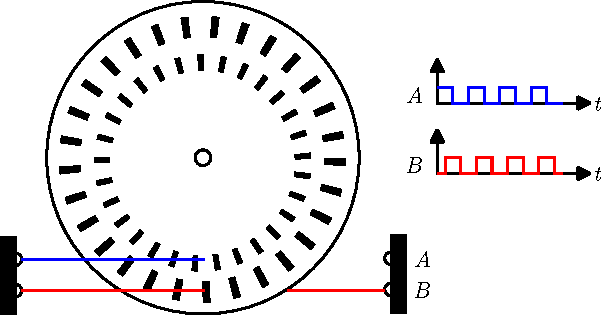
\includegraphics[width=0.6\linewidth]{master_fig/enc.pdf}
    \caption{Rotacioni enkoder.}
    \end{figure}
\end{frame}
%------------------------------------------------

\subsection{Akvizicija podataka}

\begin{frame}{Akvizicija podataka}
    \begin{figure}
    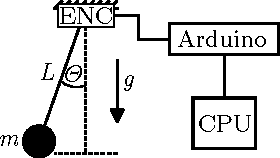
\includegraphics[width=0.6\linewidth]{master_fig/akvizicija.pdf}
    \caption{Opšta blok šema akvizicije signala sa klatna.}
    \end{figure}
\end{frame}

%------------------------------------------------

\section{Karakteristike korišćenih komponenti}

\begin{frame}
    \Huge{\centerline{\textbf{Karakteristike korišćenih komponenti}}}
\end{frame}
%------------------------------------------------

\subsection{Karakteristike klatna}

\begin{frame}{Karakteristike klatna}
    
    
    \begin{columns}[c]
    \begin{column}{.4\textwidth}
    \centering		 
    		 1. Tegovi \\
    		 2. Neistegljive šipke \\
    		 3. Opruga \\
    		 4. Enkoderi \\
    		 5. Prenosni sistem
    \end{column}
    \begin{column}{.6\textwidth}
    \begin{figure}
    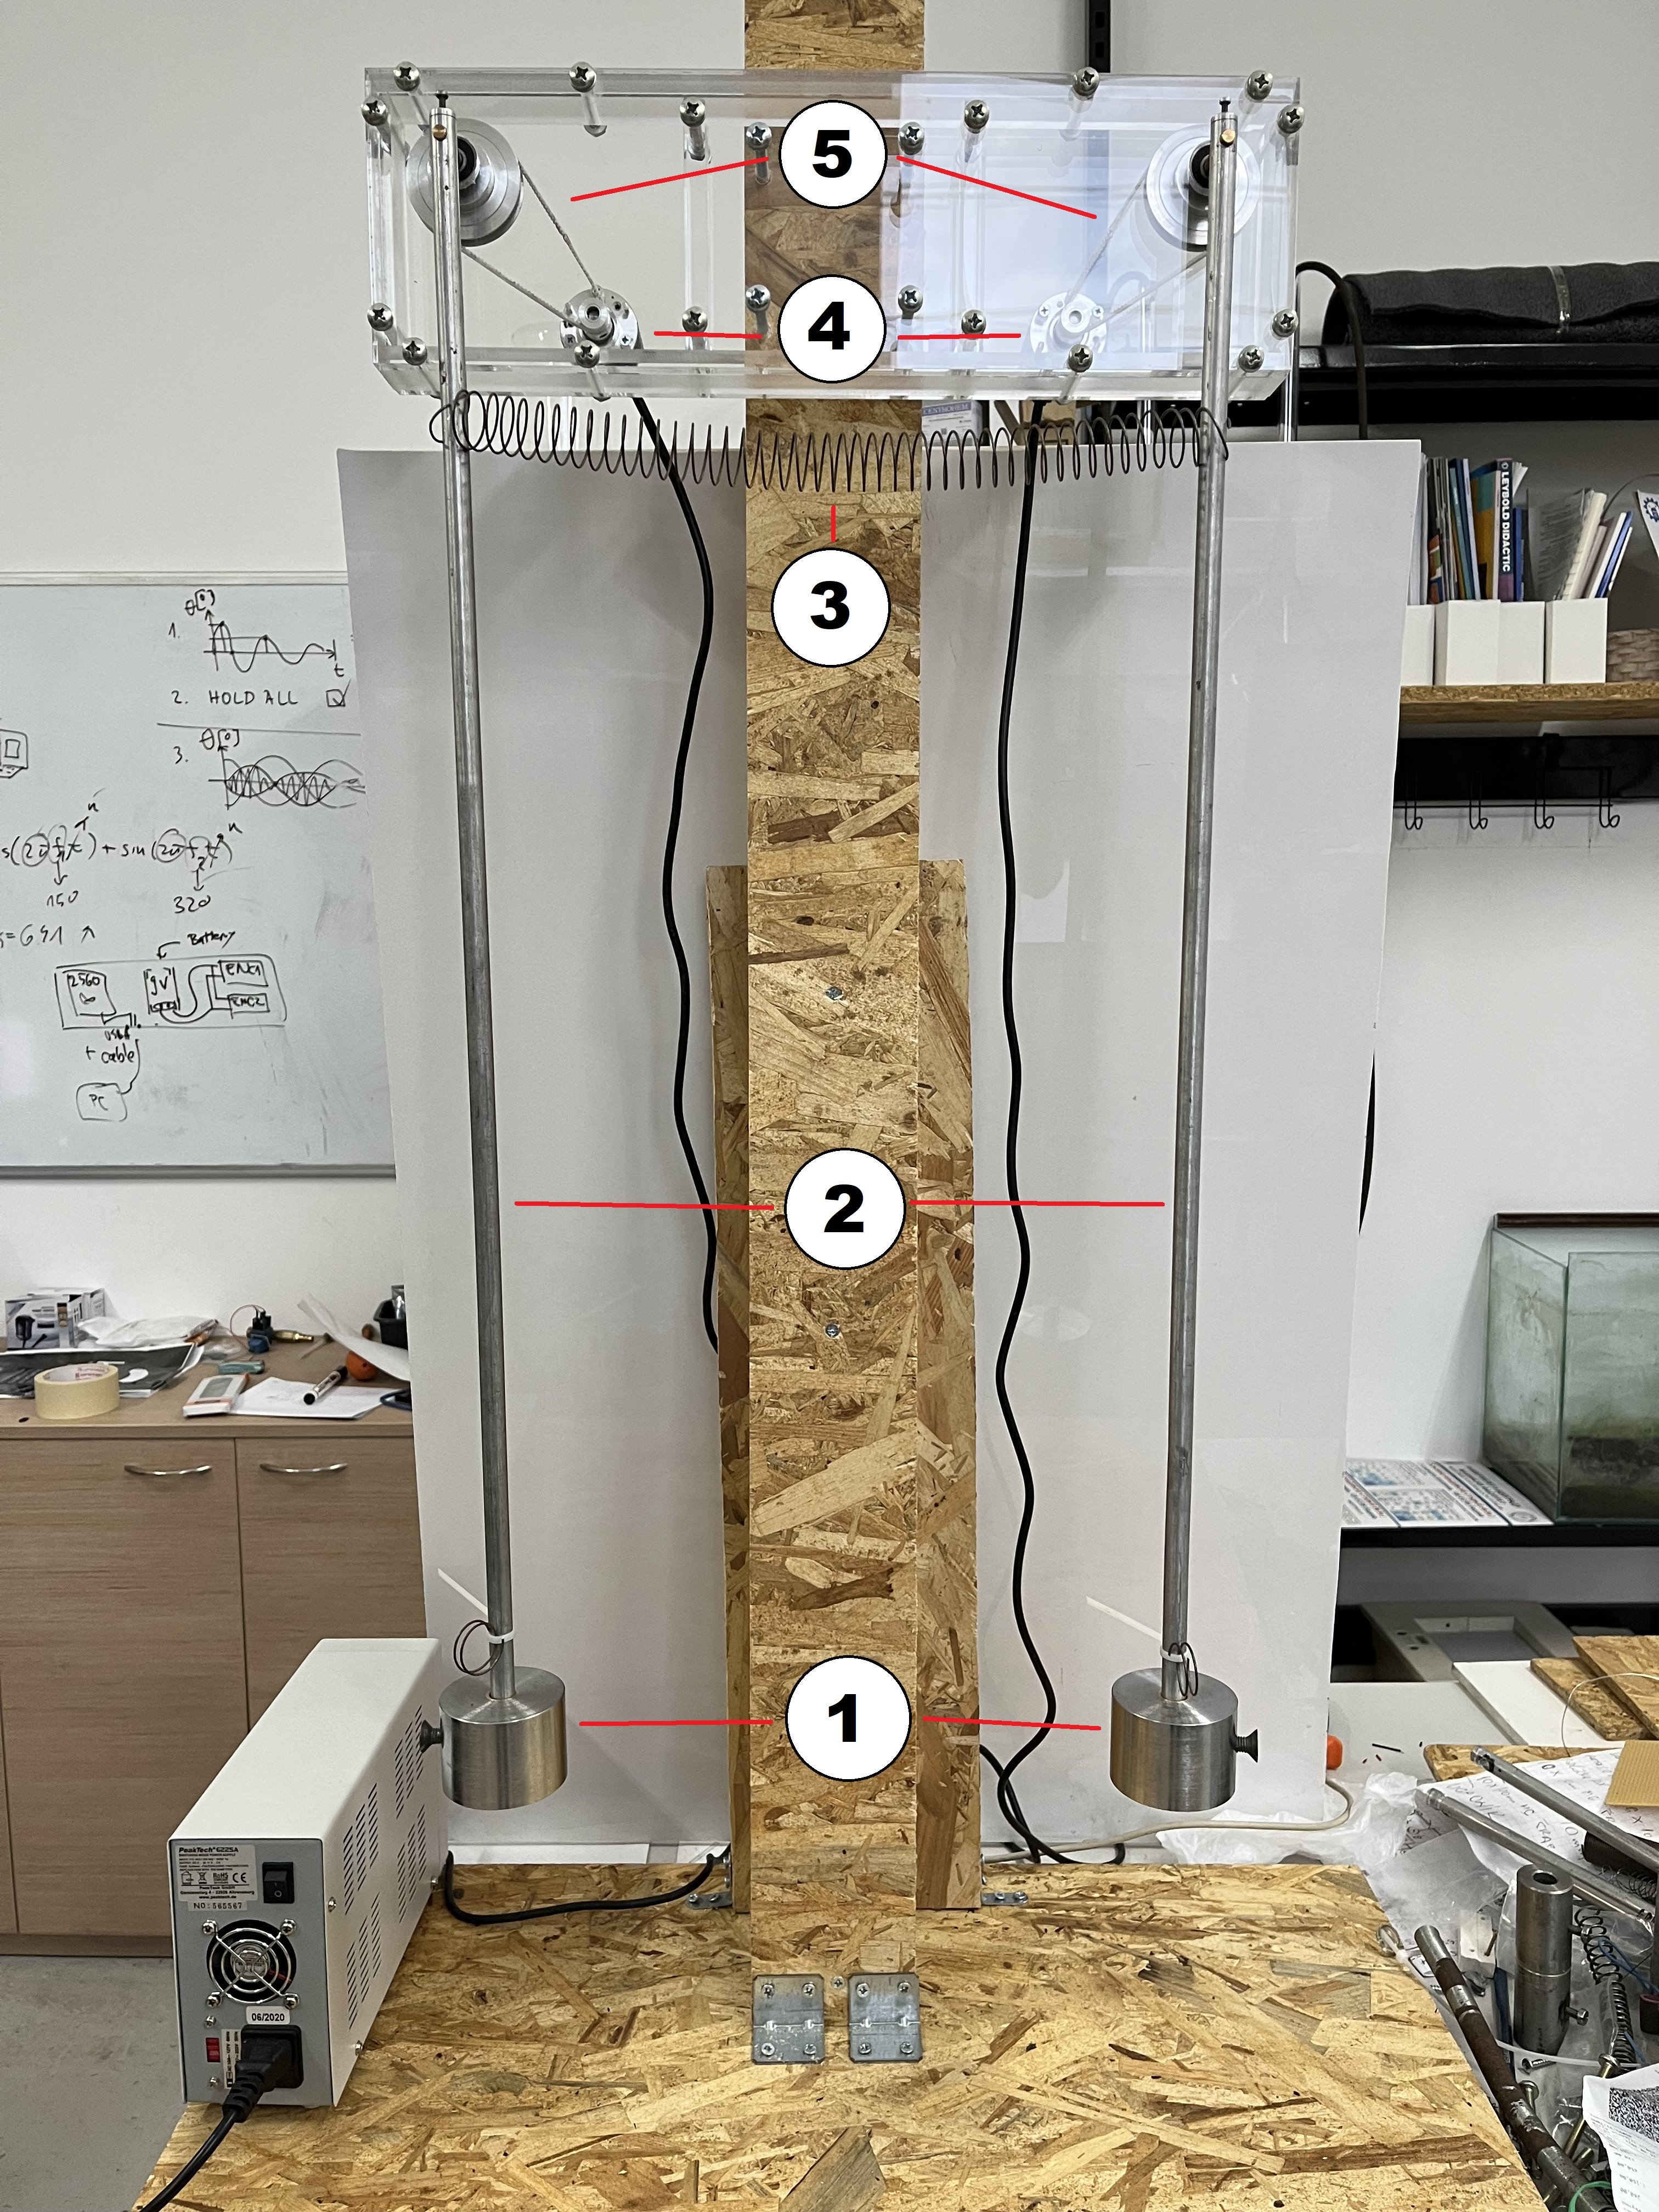
\includegraphics[width=0.5\linewidth]{master_fig/klatno2.jpeg}
    \caption{Eksperimentalna postavka spregnutih klatana.}
    \end{figure}
    \end{column}
\end{columns}
    
    
\end{frame}

%------------------------------------------------

\subsection{Sistem za prenos}

\begin{frame}{Sistem za prenos}
    
    
    \begin{columns}[c]
    \begin{column}{.4\textwidth}
    \centering		 
    		 1. Enkoder sa manjim zupčanikom \\
    		 2. Druga osovina sa većim zupčanikom \\
    		 3. Neistegljivi zupčasti kaiš za povezivanje \\
    \end{column}
    \begin{column}{.6\textwidth}
    \begin{figure}
    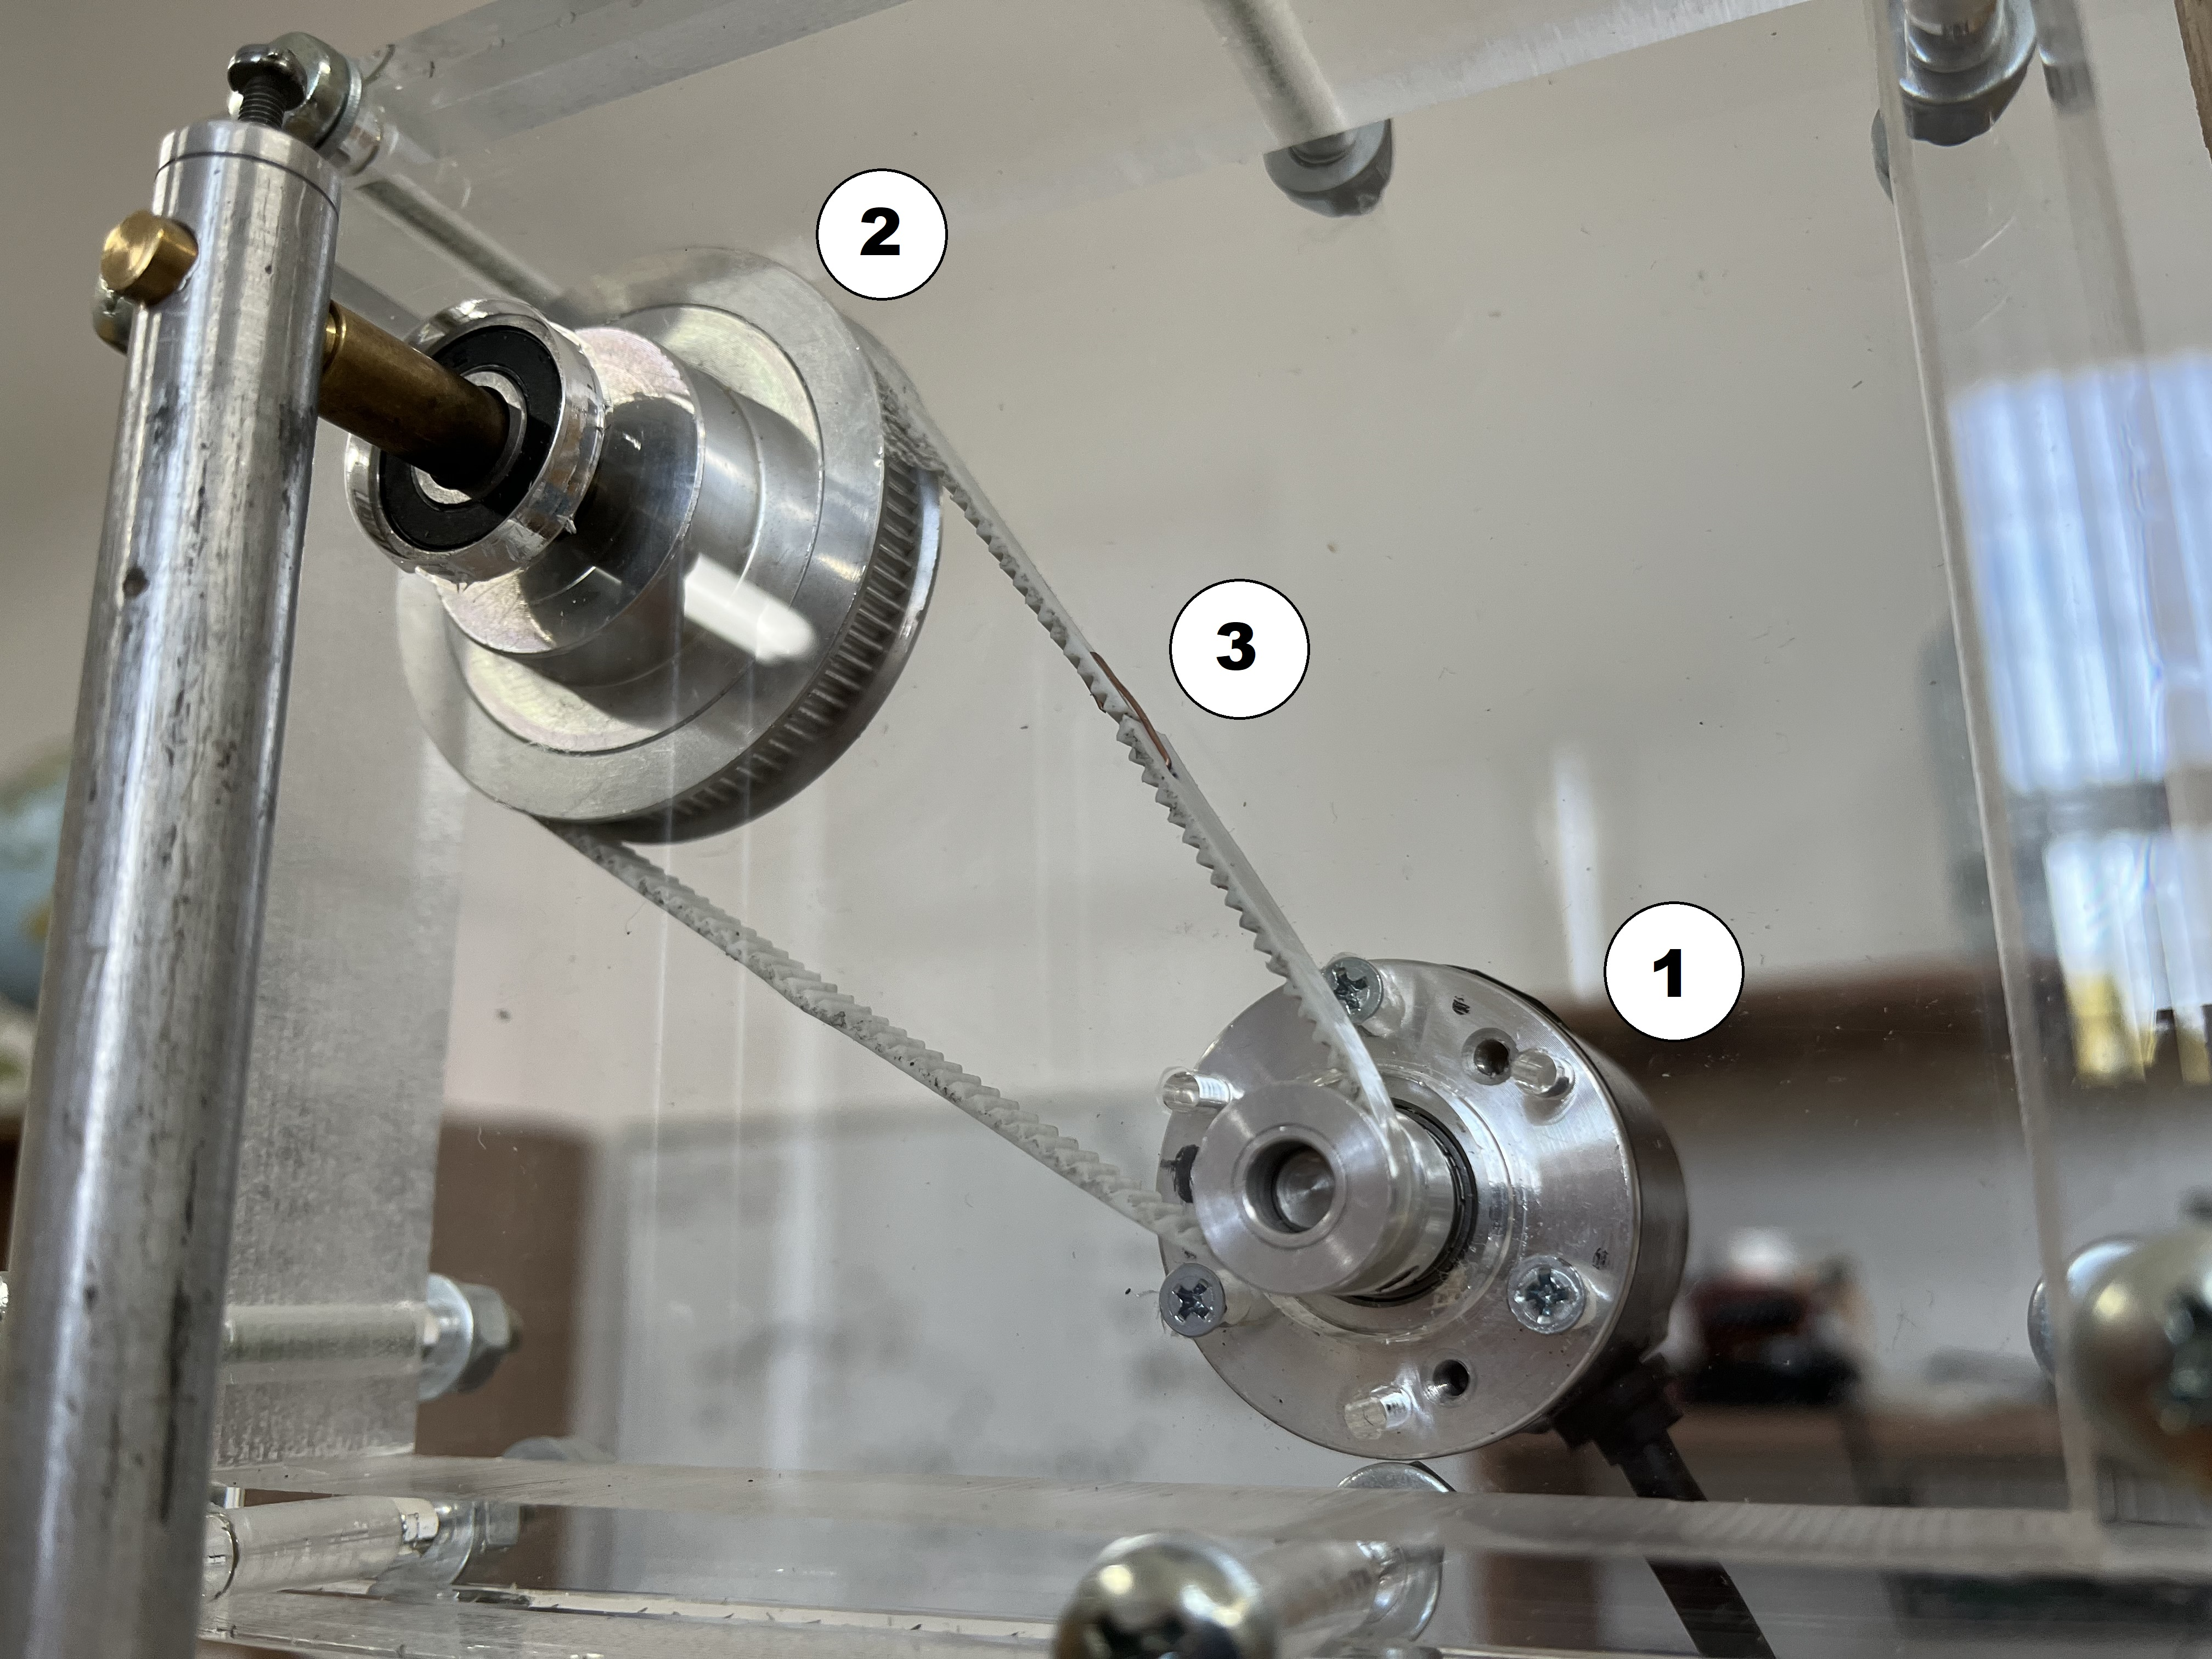
\includegraphics[width=0.8\linewidth]{master_fig/prenos2.jpeg}
    \caption{Sistem za prenos.}
    \end{figure}
    \end{column}
\end{columns}
    
    
\end{frame}

%------------------------------------------------

\subsection{Karakteristike enkodera}

\begin{frame}{Karakteristike enkodera}
    \begin{figure}
    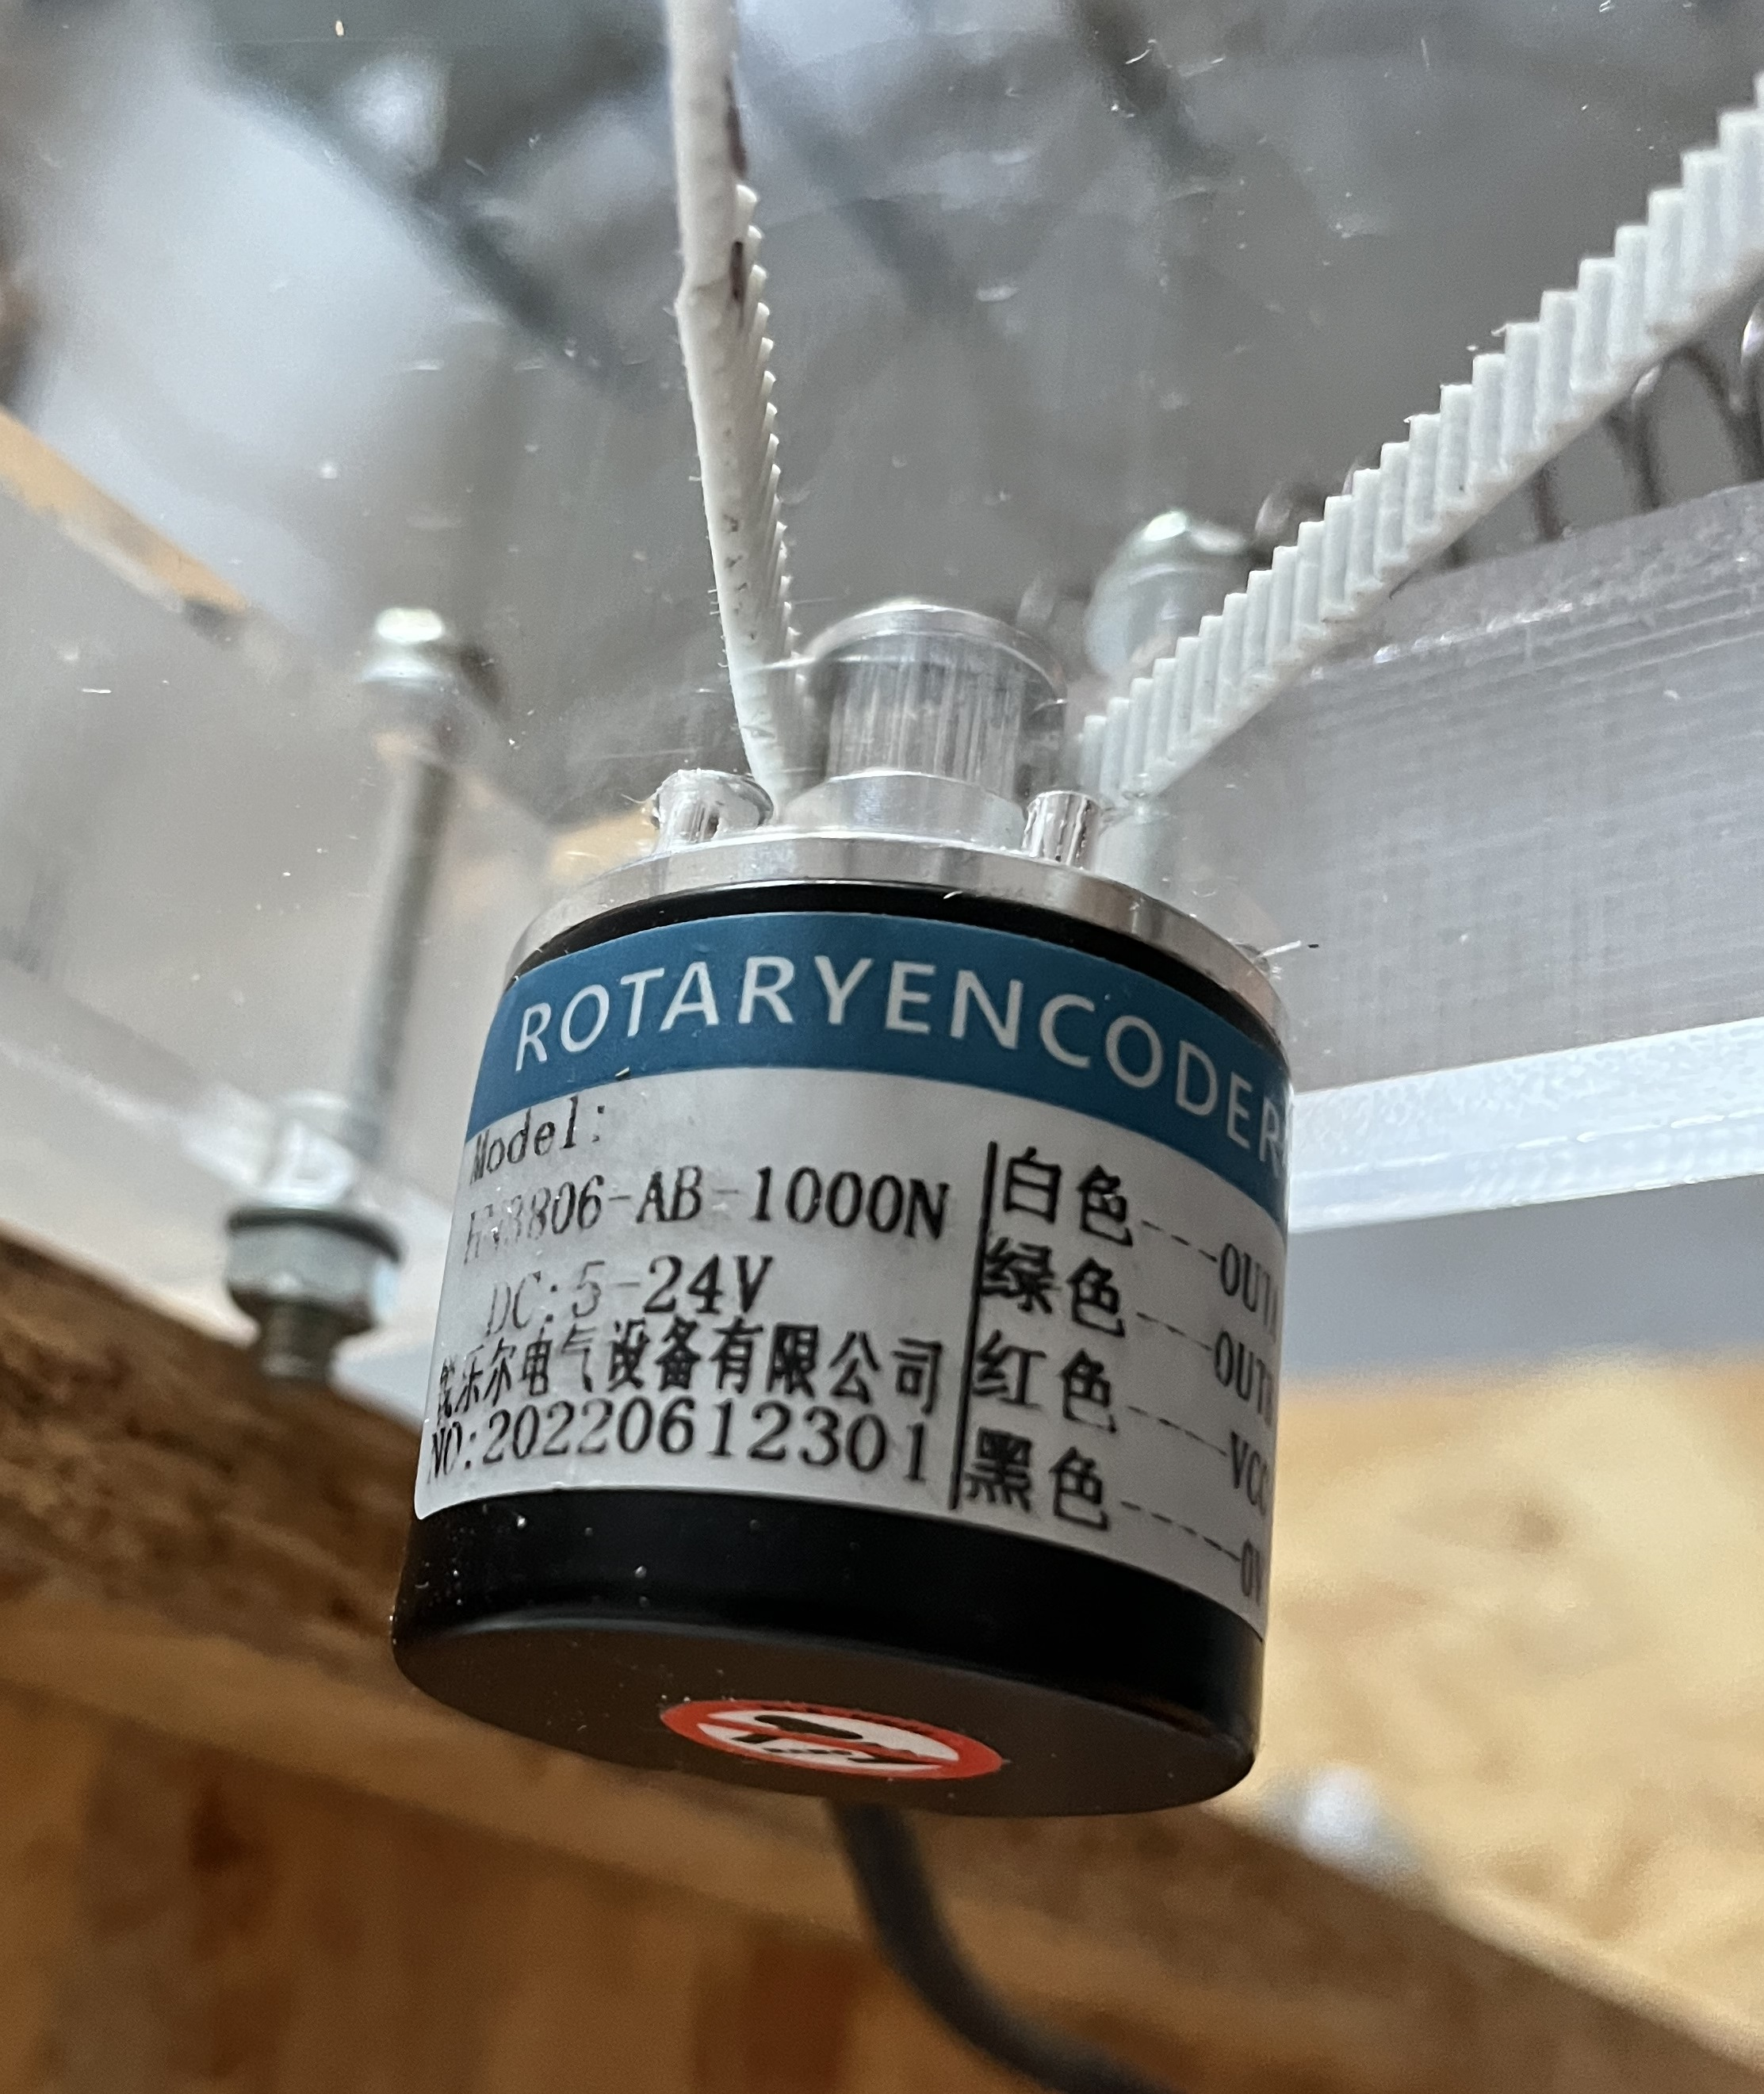
\includegraphics[width=0.3\linewidth]{master_fig/enc2.jpeg}
    \caption{Enkoder.}
    \end{figure}
\end{frame}

%------------------------------------------------

\subsection{Napajanje}

\begin{frame}{Napajanje}
    \begin{figure}
    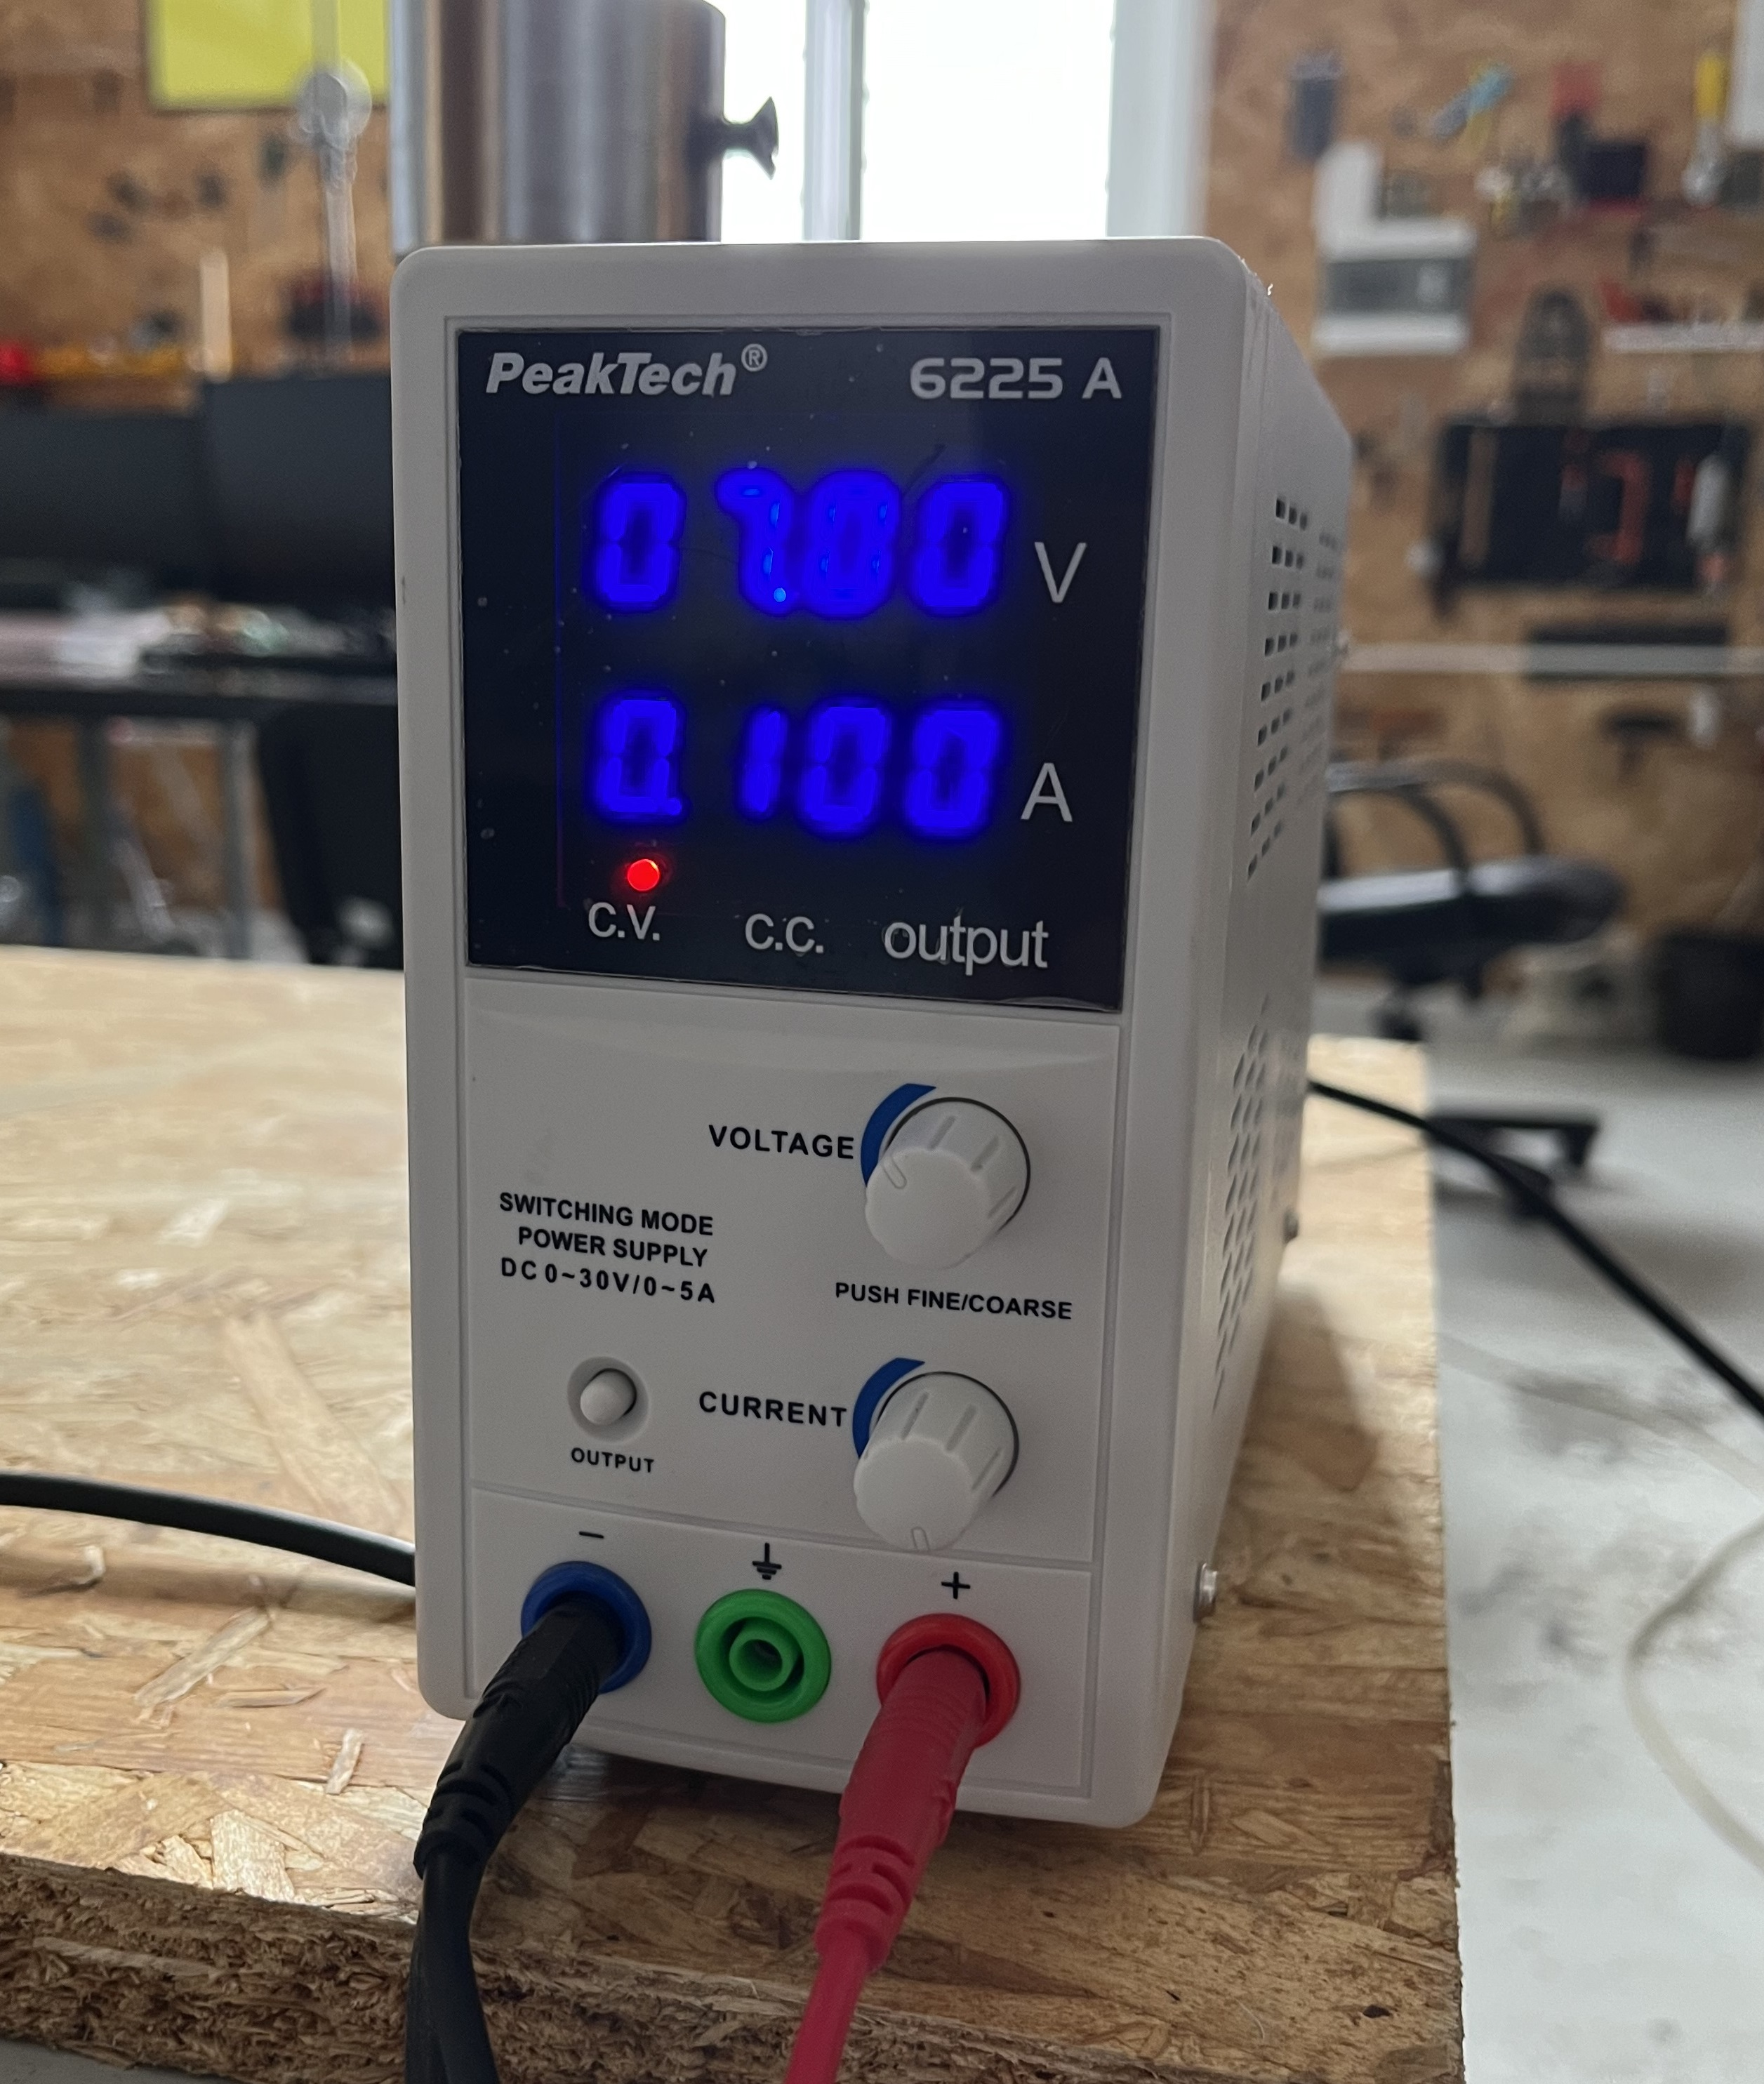
\includegraphics[width=0.3\linewidth]{master_fig/peaktech2.jpeg}
    \caption{Eksterno napajanje.}
    \end{figure}
\end{frame}

%------------------------------------------------

\begin{frame}{Portabilno eksterno napajanje}
	\begin{columns}[c]
    \begin{column}{.45\textwidth}
    \begin{figure}
        \centering
        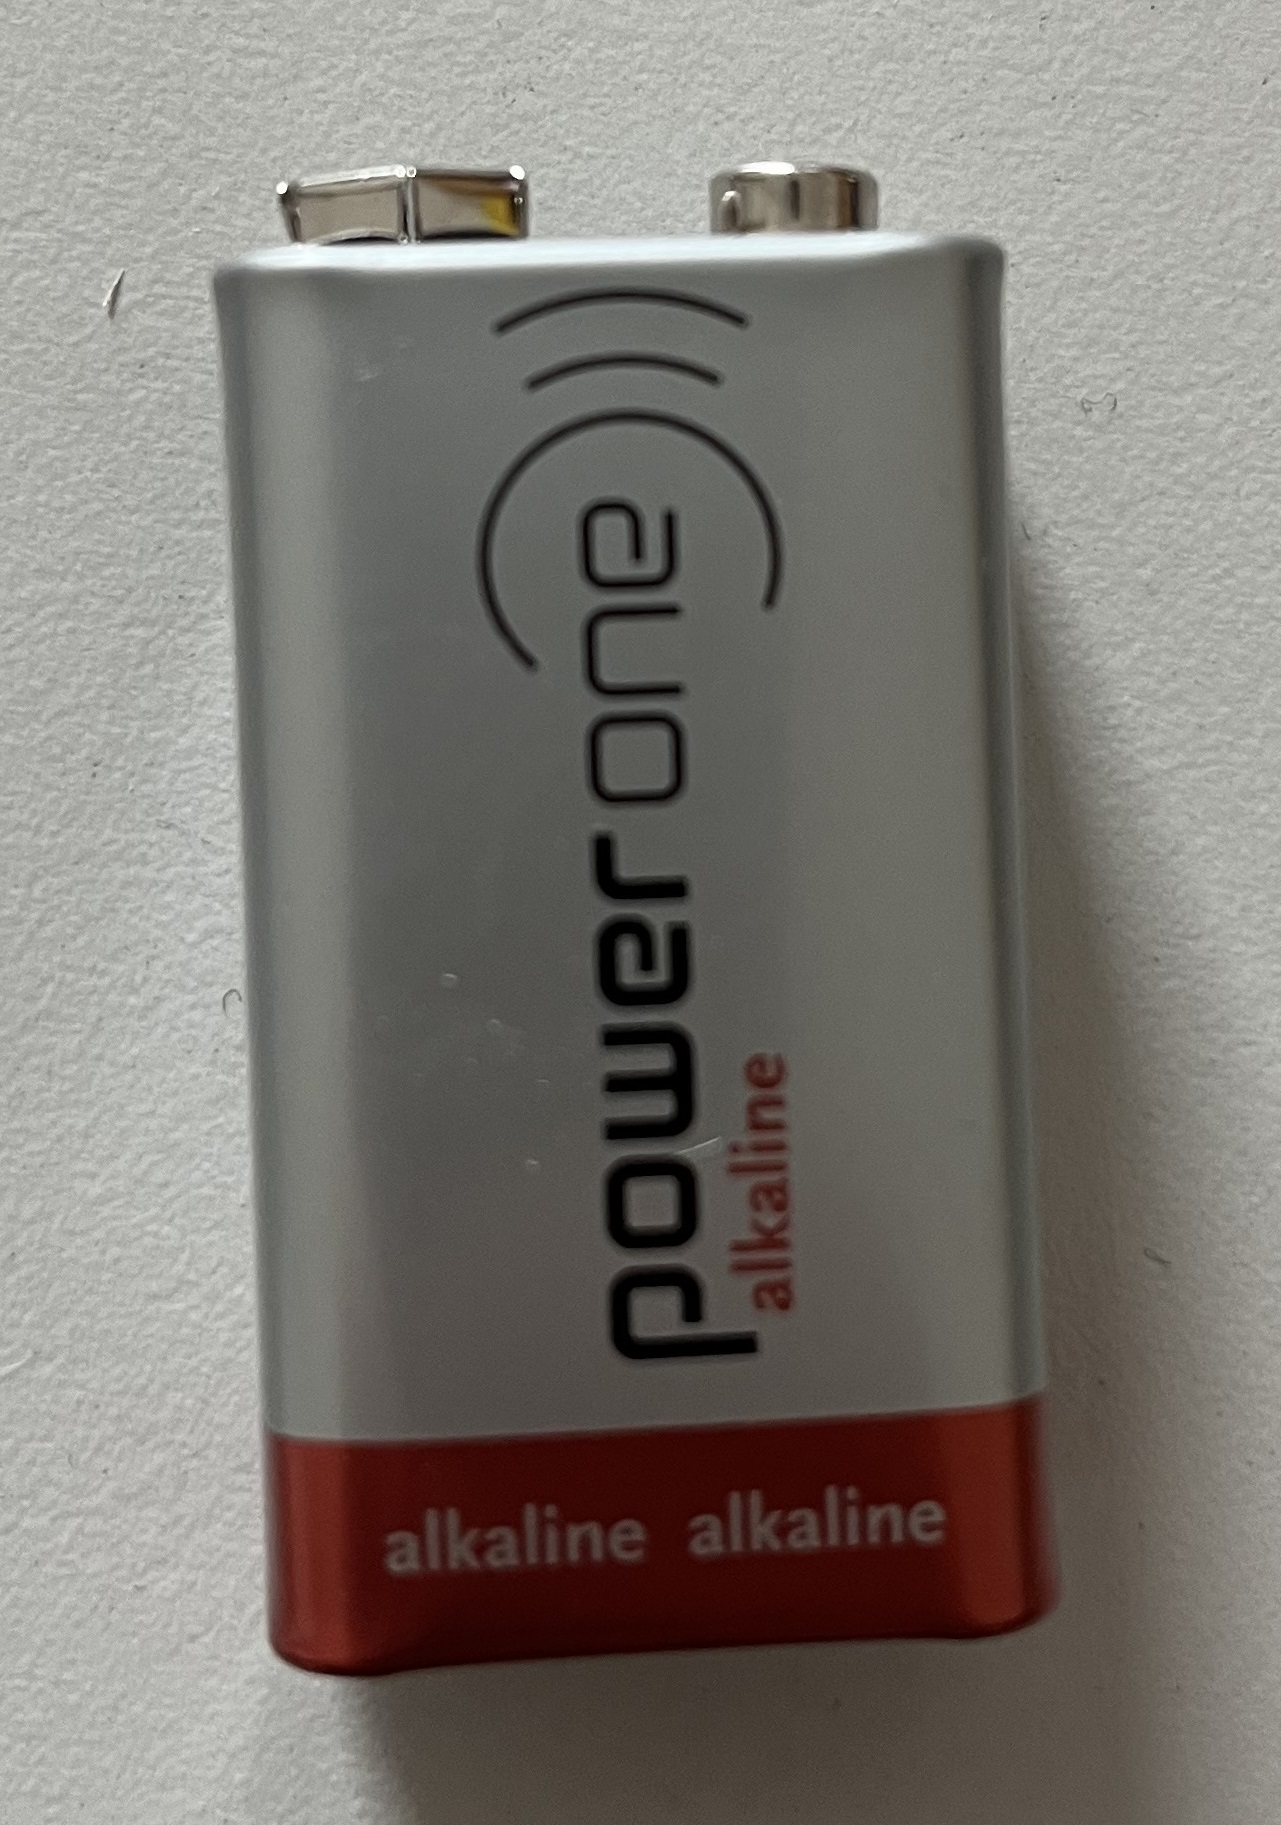
\includegraphics[width=0.6\textwidth]{master_fig/baterija2.jpeg}
        \caption{Baterija.}
    \end{figure}      
    \end{column}
    \begin{column}{.55\textwidth}
    \begin{figure}
        \centering
        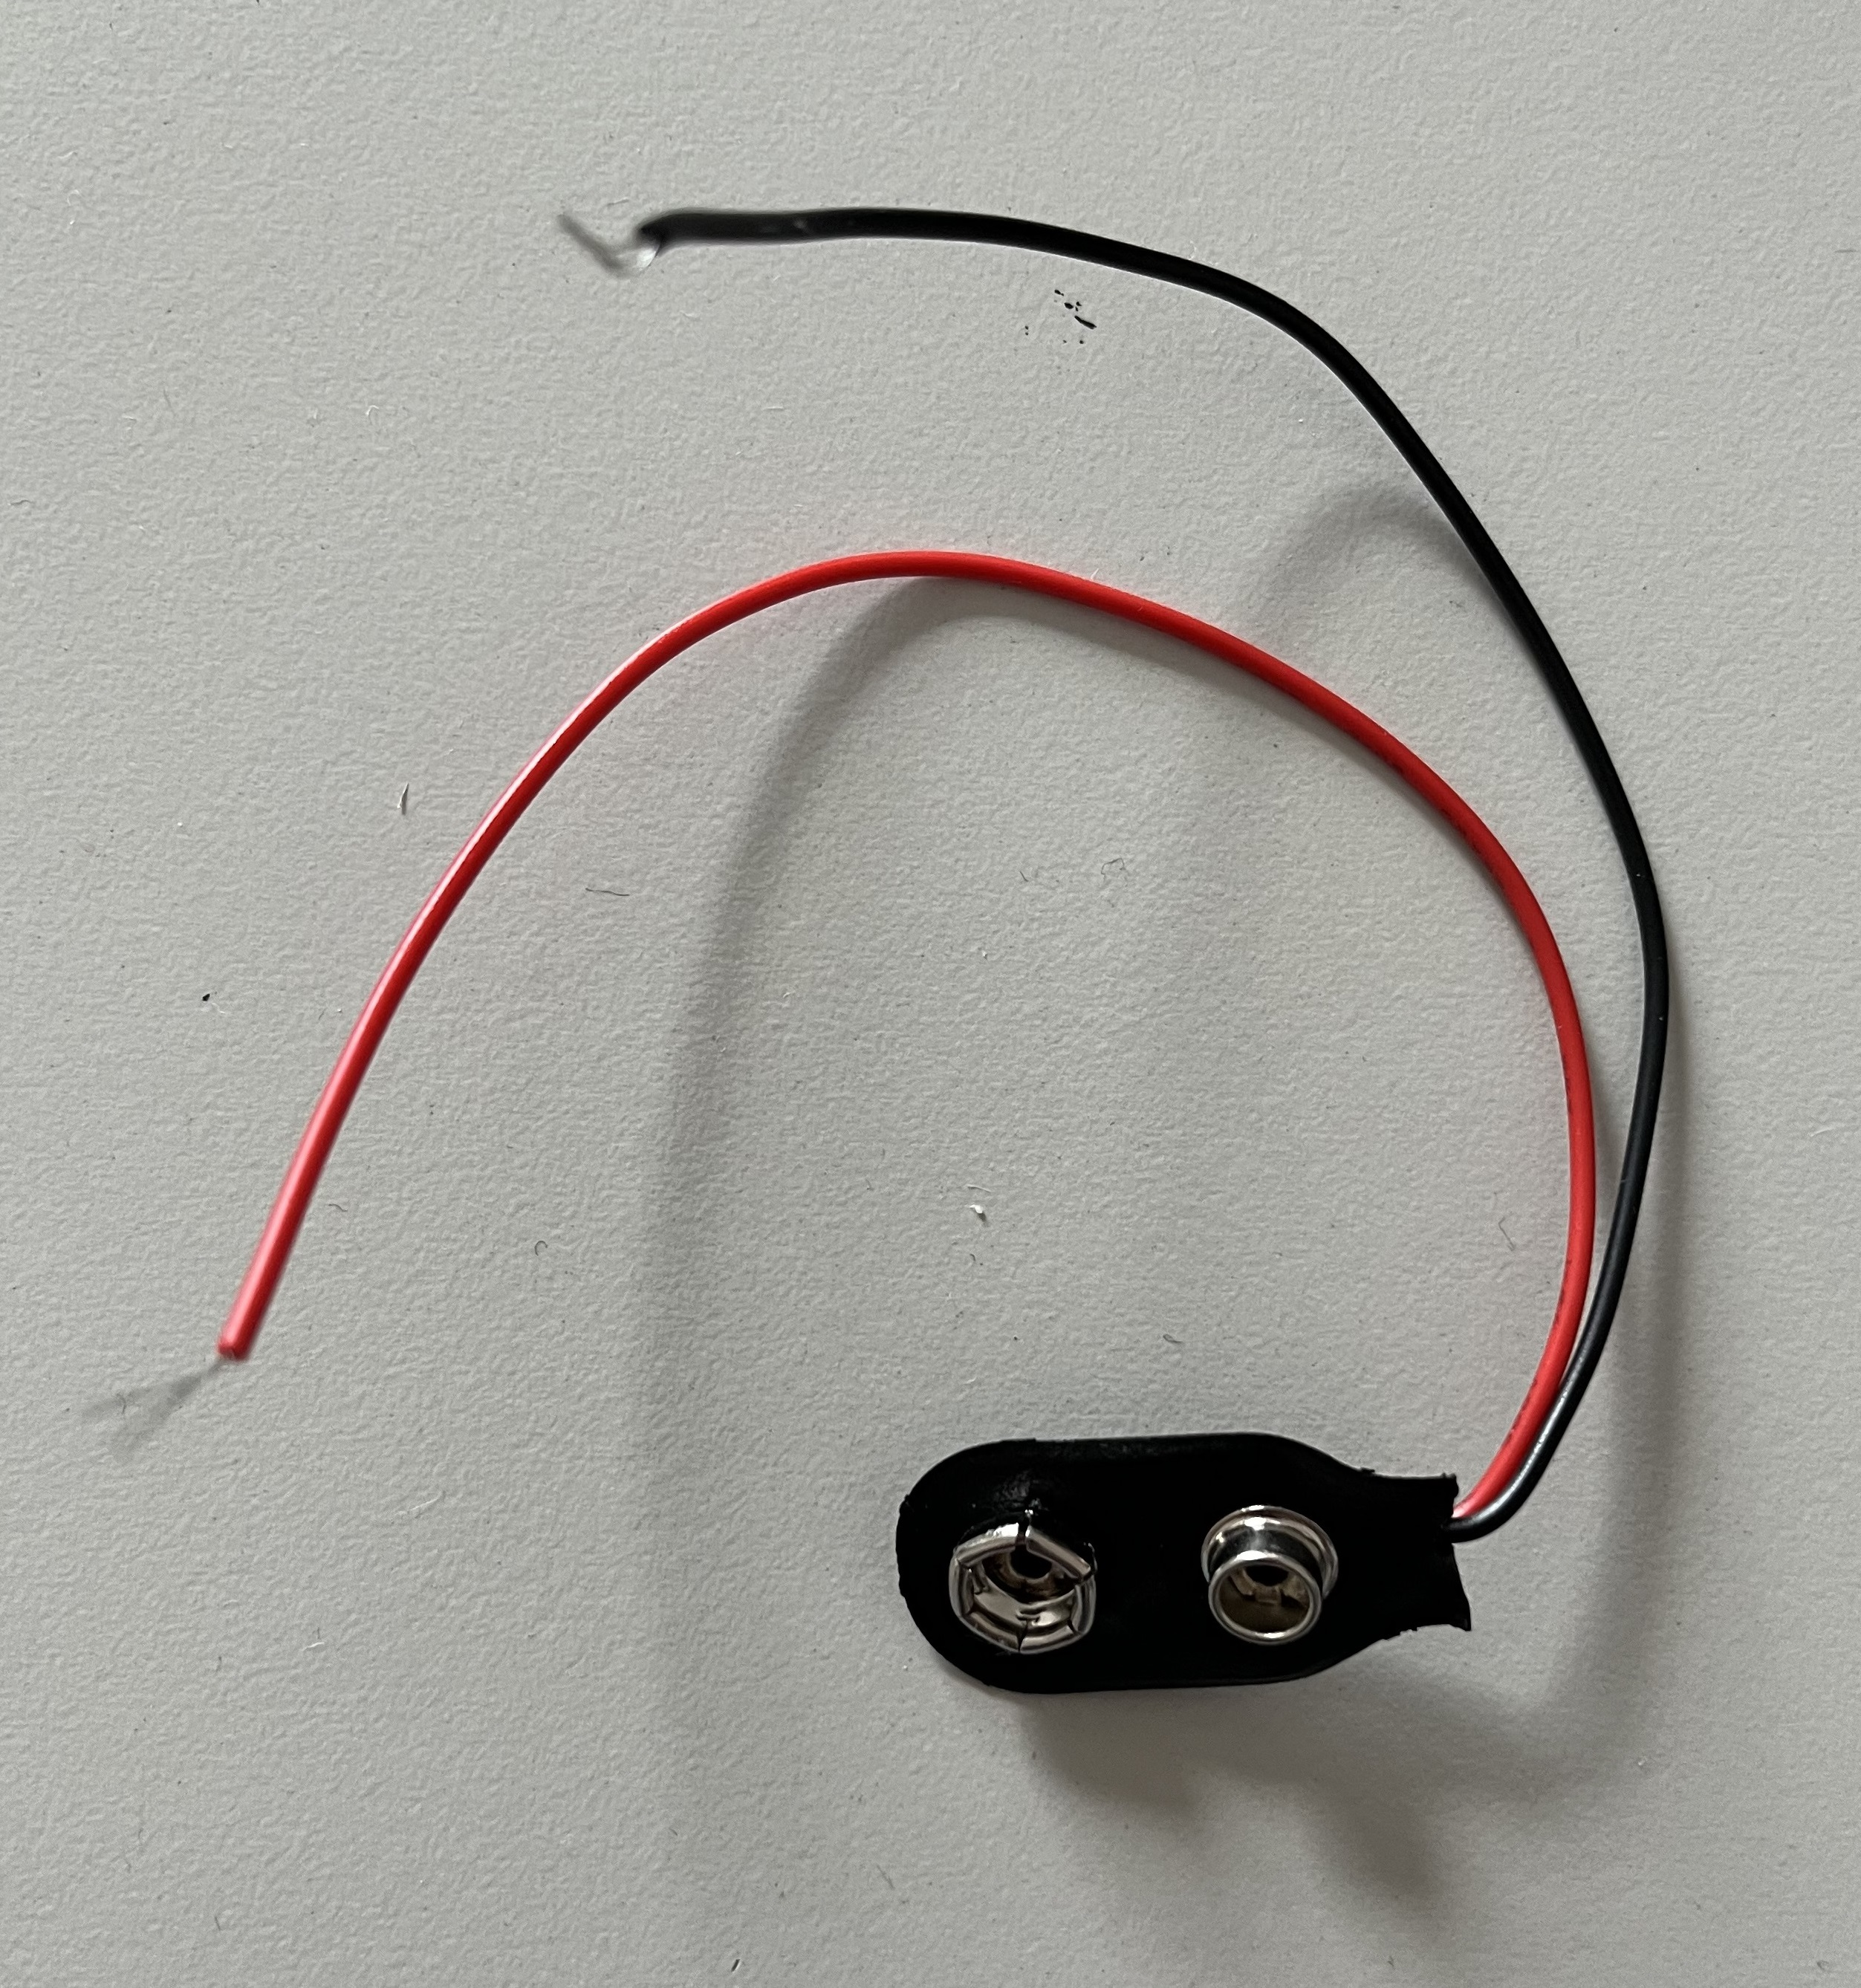
\includegraphics[width=0.65\textwidth]{master_fig/konektor3.jpeg}
        \caption{Konektor za bateriju.}
    \end{figure}
    \end{column}
\end{columns}
\end{frame}

%------------------------------------------------

\subsection{Karakteristike Arduina}

\begin{frame}{Arduino Mega 2560}
    \begin{figure}
    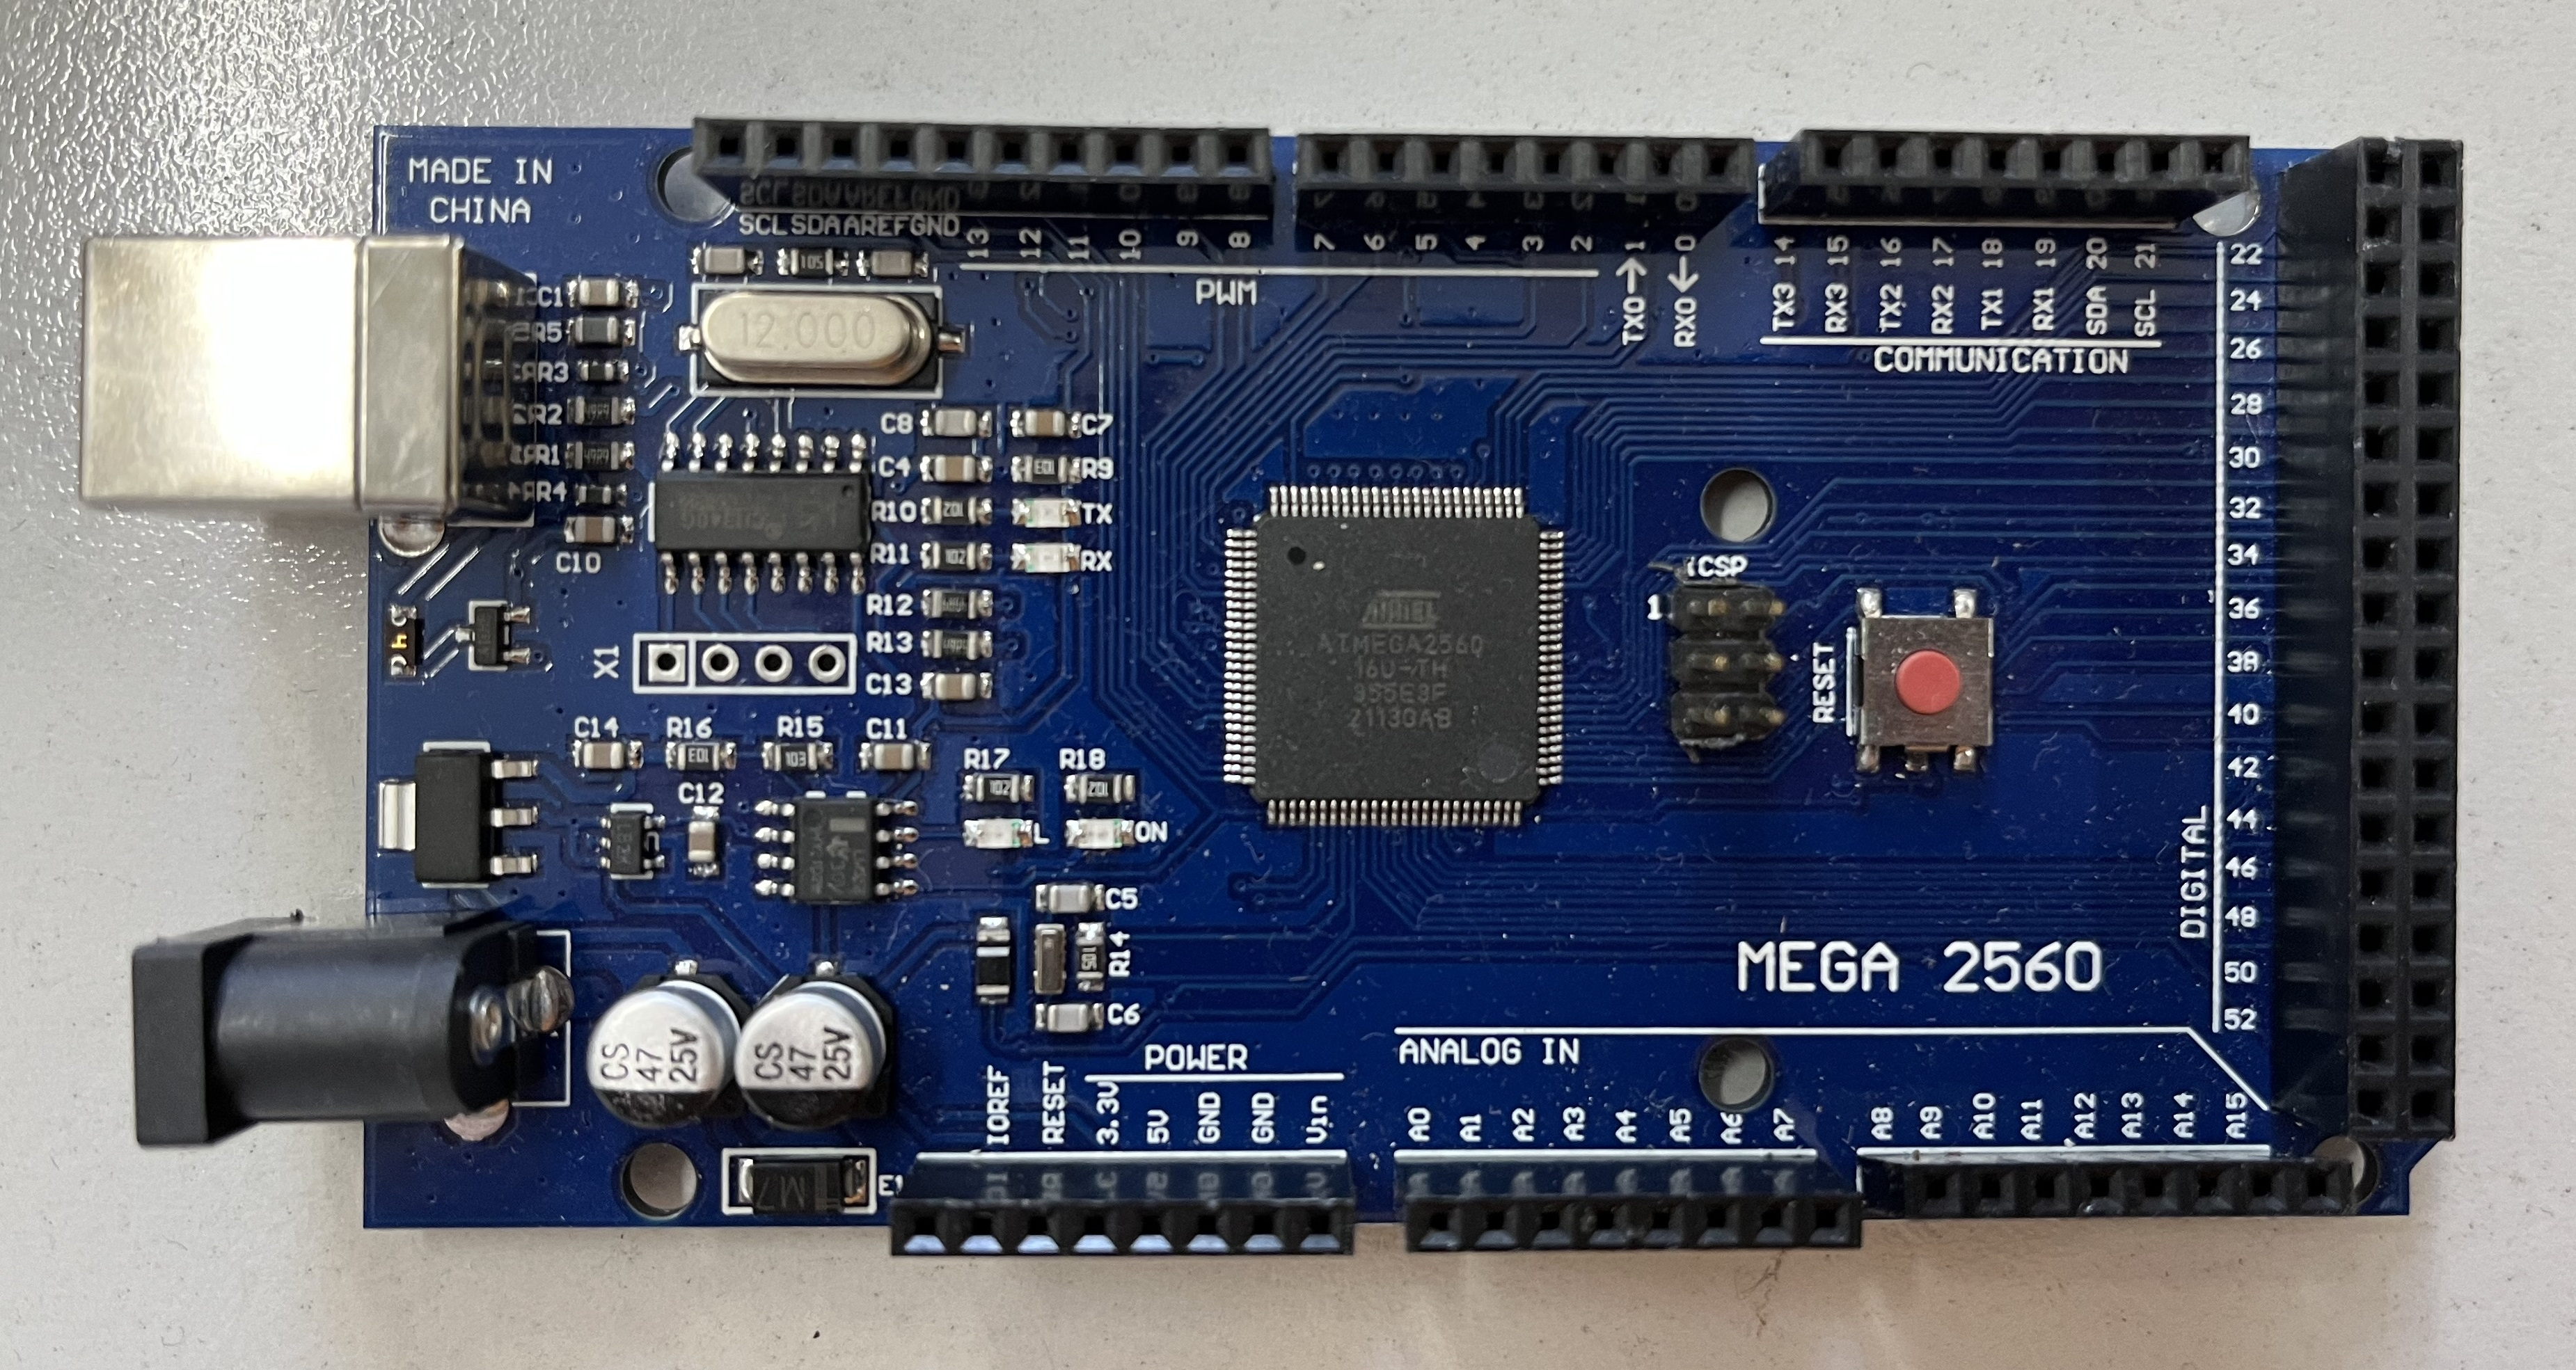
\includegraphics[width=0.75\linewidth]{master_fig/mega2560_2.jpeg}
    \caption{Arduino Mega 2560.}
    \end{figure}
\end{frame}

%------------------------------------------------

\begin{frame}{Radno merno okruženje}
    \begin{figure}
    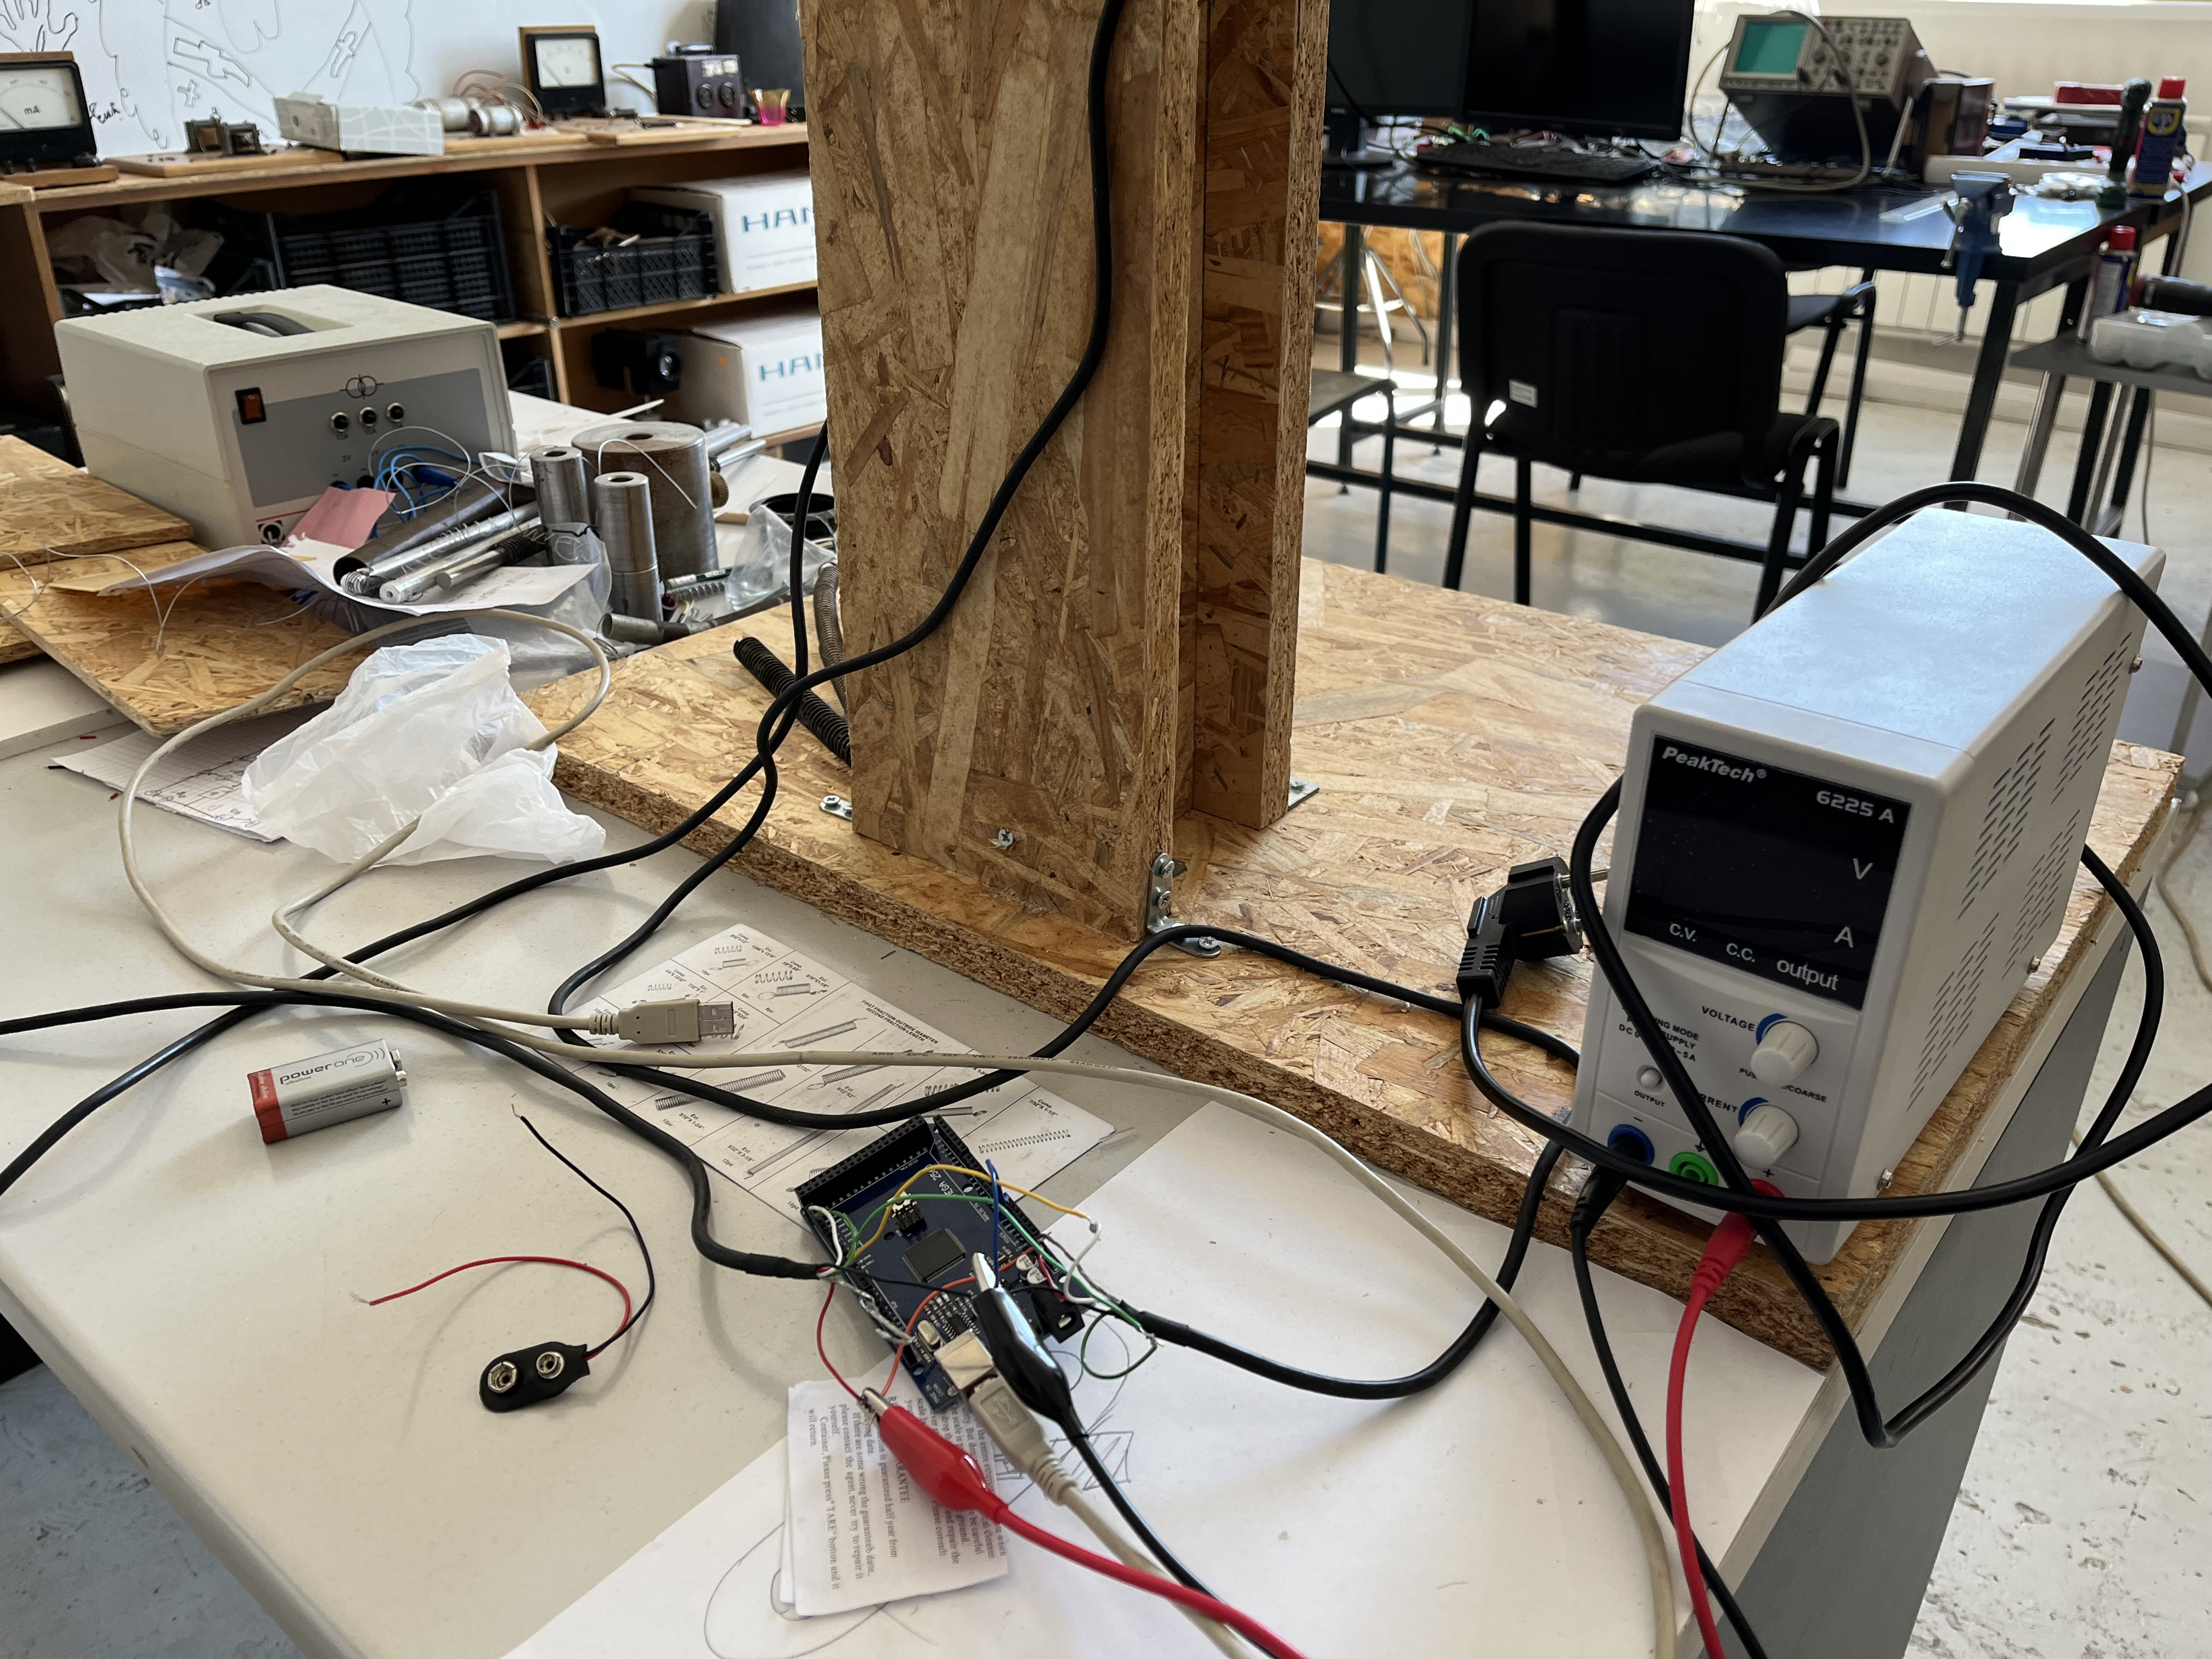
\includegraphics[width=0.6\linewidth]{fig/img/lab.jpeg}
    \caption{Radno okruženje sa projektovanim sistemom i aparaturom za merenje (Lab 24).}
    \end{figure}
\end{frame}

%------------------------------------------------

\section{Rezultati i diskusija}

\begin{frame}
    \Huge{\centerline{\textbf{Rezultati i diskusija}}}
\end{frame}

%------------------------------------------------

\begin{frame}{Rezultati merenja}
    \begin{figure}
    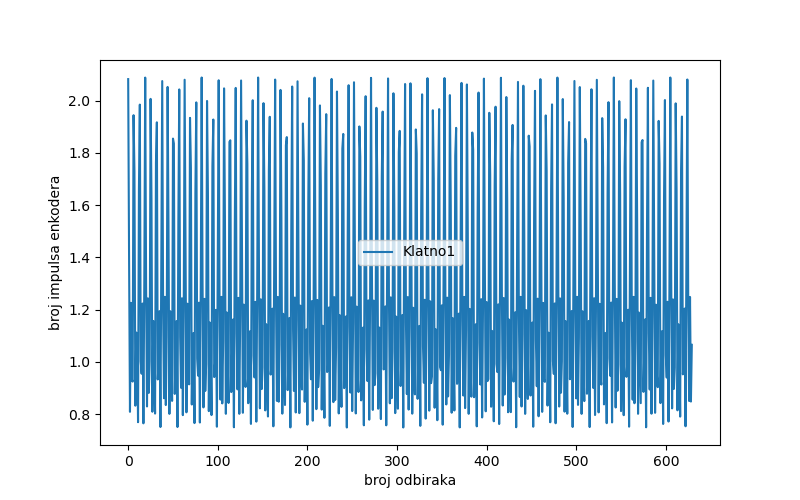
\includegraphics[width=0.65\linewidth]{master_fig/klatno_0.png}
    \caption{Rezultati inicijalnog merenja, Arduino Uno, bez prenosa.}
    \end{figure}
\end{frame}

%------------------------------------------------
\begin{frame}{Rezultati merenja}
    \begin{figure}
    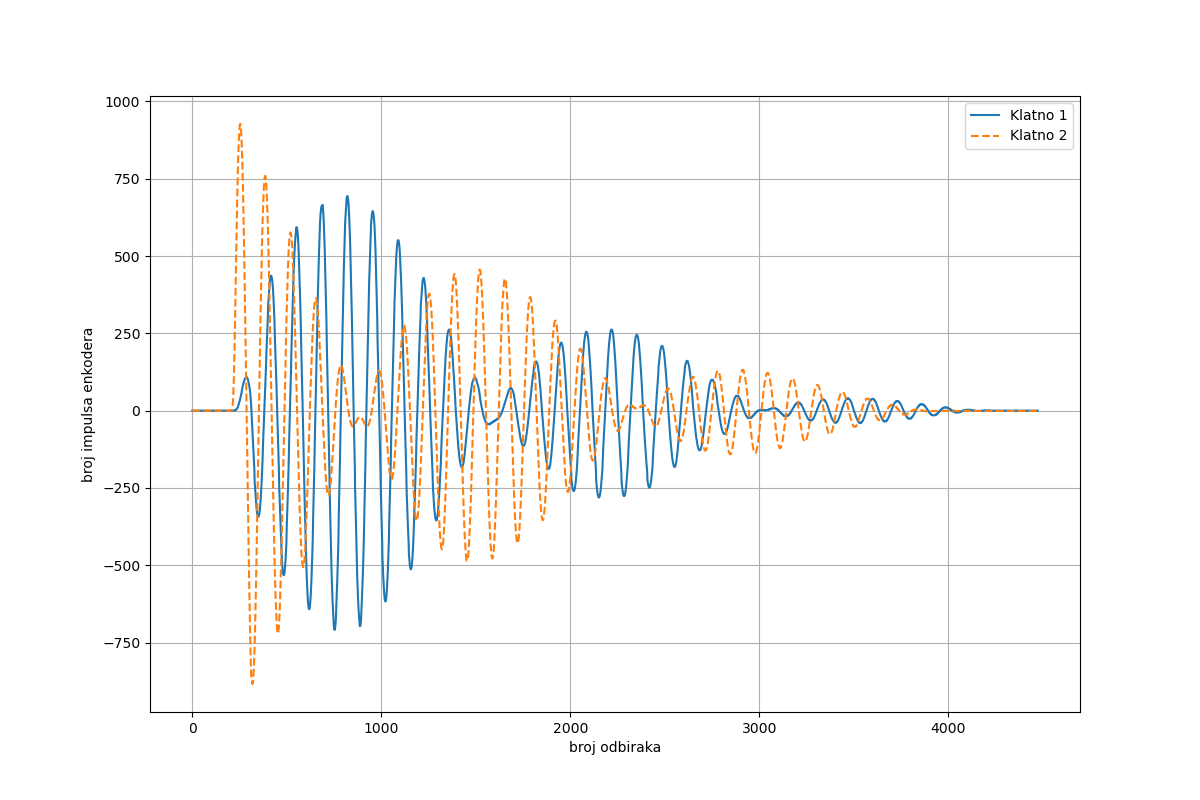
\includegraphics[width=0.65\linewidth]{master_fig/klatno.png}
    \caption{Rezultati merenja prve postavke, Arduino Mega 2560, bez prenosa.}
    \end{figure}
\end{frame}


%------------------------------------------------
\begin{frame}{Rezultati merenja}
    \begin{figure}
    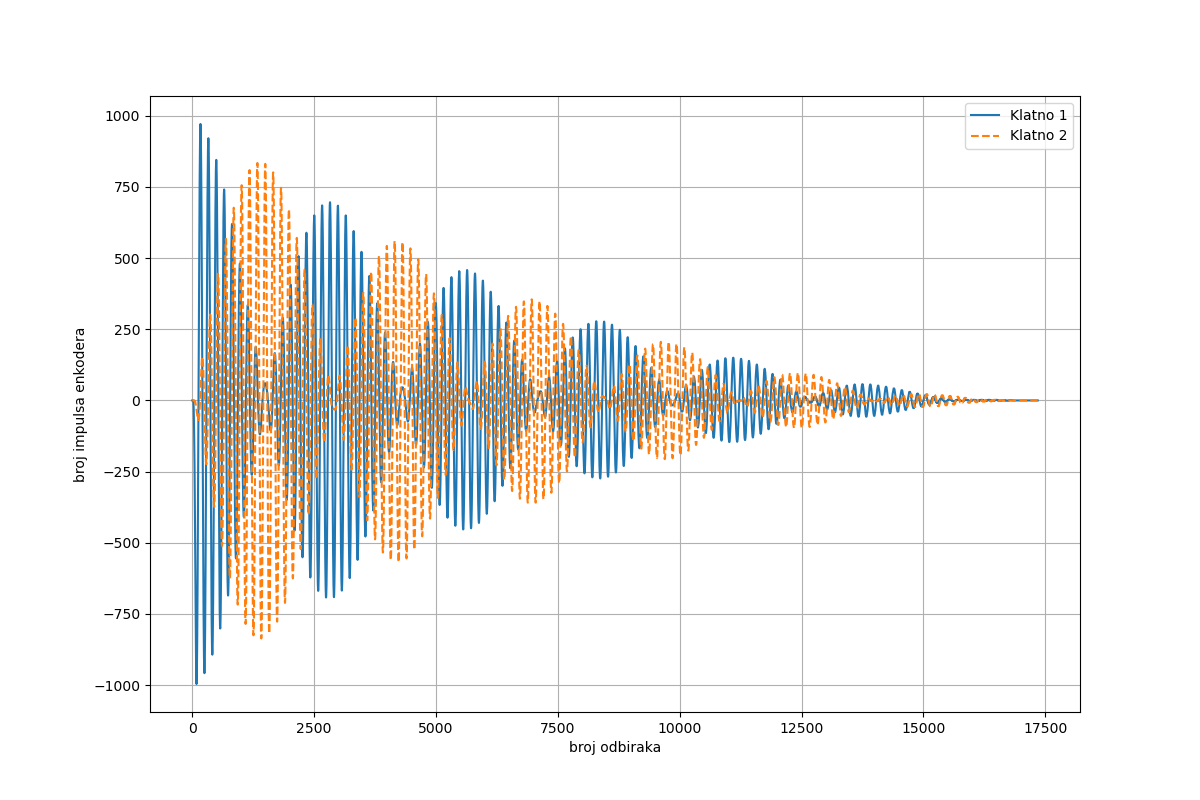
\includegraphics[width=0.65\linewidth]{master_fig/klatno_2.png}
    \caption{Rezultati merenja finalne postavke, Arduino Mega 2560, sa prenosom.}
    \end{figure}
\end{frame}


%------------------------------------------------
\begin{frame}{Rezultati merenja}
    \begin{figure}
    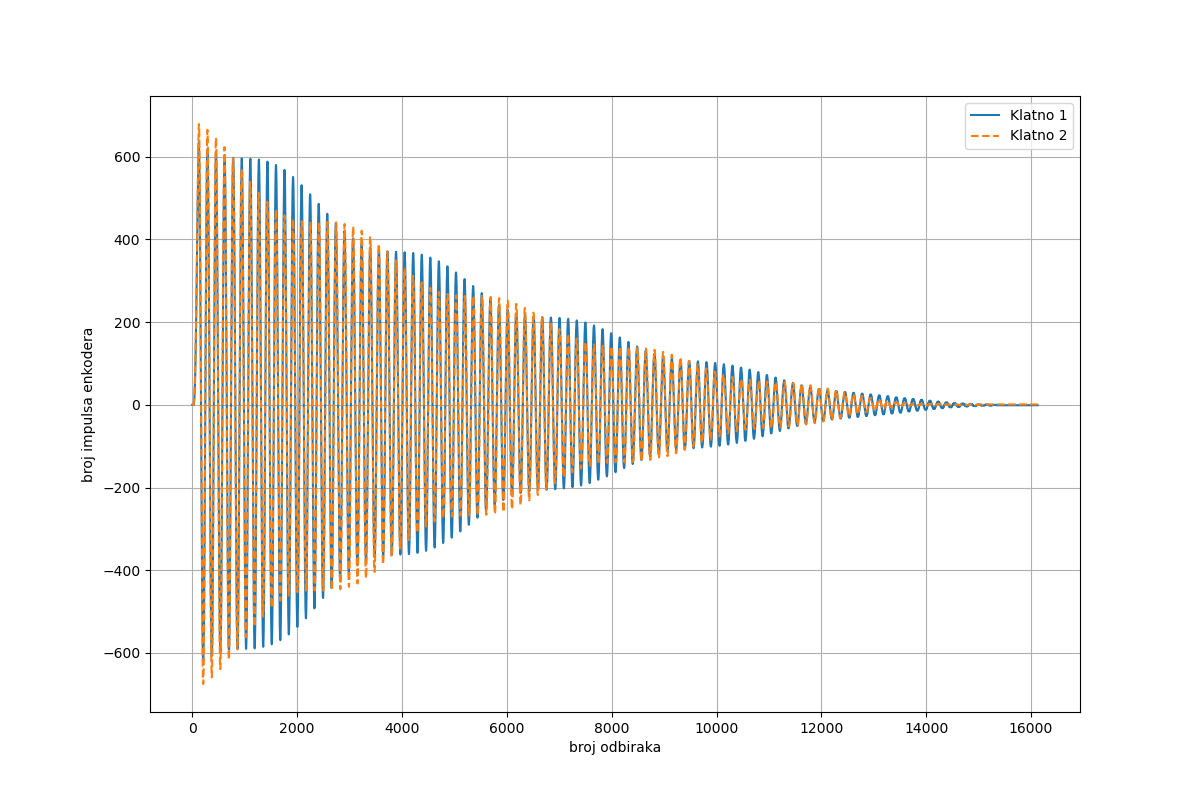
\includegraphics[width=0.65\linewidth]{master_fig/klatno_sim.png}
    \caption{Rezultati merenja finalne postavke, mod simetrije.}
    \end{figure}
\end{frame}


%------------------------------------------------
\begin{frame}{Rezultati merenja}
    \begin{figure}
    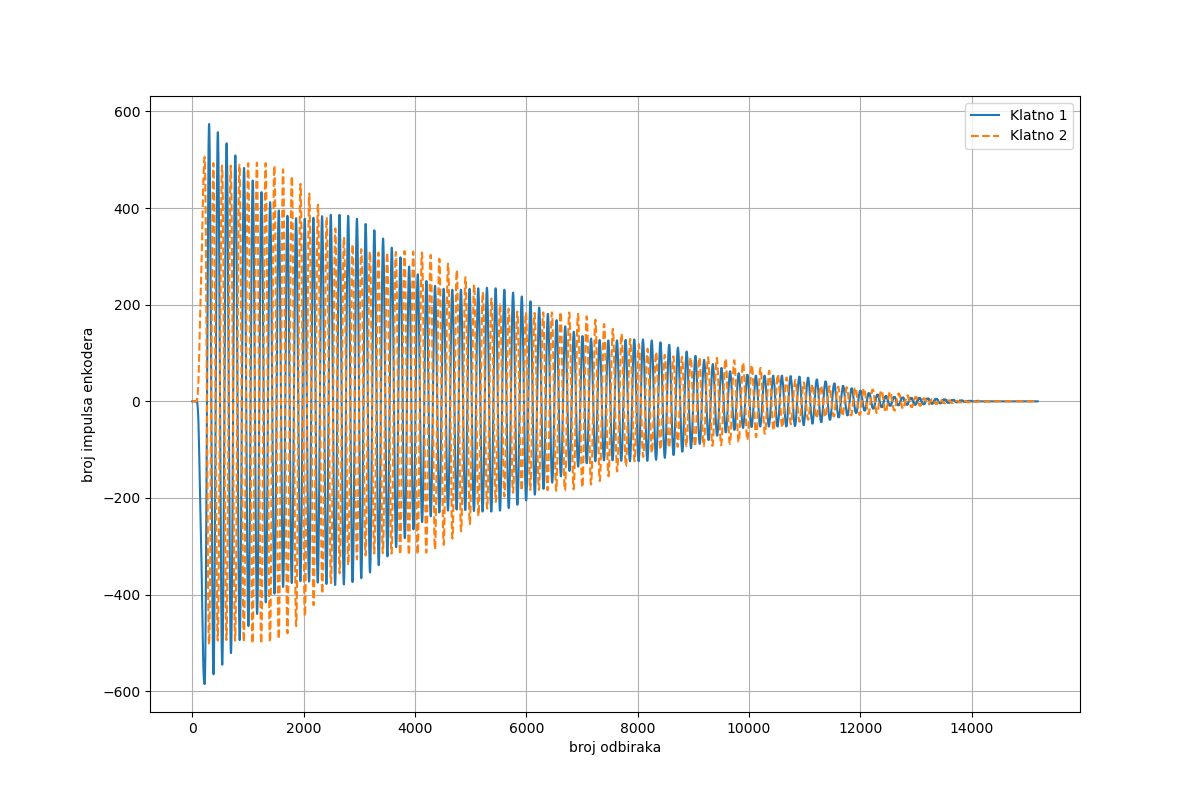
\includegraphics[width=0.65\linewidth]{master_fig/klatno_antisim.png}
    \caption{Rezultati merenja finalne postavke, mod antisimetrije.}
    \end{figure}
\end{frame}


%------------------------------------------------

\begin{frame}{Zaključak}

	\begin{itemize}
		\item Teorija - modeli - merenja
		\item Upotreba
		\item Preporuke za dalje modifikacije
			\begin{itemize}
				\item Automatizacija pozicioniranja klatna
				\item Daljinska kontrola
				\item senzori za napajanje
			\end{itemize}
		
	\end{itemize}
    
\end{frame}



\begin{frame}

	\Huge{{\centerline{\textbf{Zahvalnost}}}}
    
\end{frame}


\begin{frame}

	\Huge{{\centerline{\textbf{Hvala na pažnji!}}}}
    
\end{frame}

%------------------------------------------------



%----------------------------------------------------------------------------------------

\end{document}